% Copyright 2012 by Joseph Pan <cs.wzpan@gmail.com>
%
% This file may be distributed and/or modified
%
% 1. under the LaTeX Project Public License and/or
% 2. under the GNU Public License.
%
% See the file doc/licenses/LICENSE for more details.


\documentclass[xcolor=svgnames]{beamer}

% set figure path
\graphicspath{{figures/}}


% Standard packages

\usepackage[english]{babel}
\usepackage[latin1]{inputenc}
\usepackage{times}
\usepackage[T1]{fontenc}
\usepackage{tabularx,multirow,multicol,keystroke,subfigure,longtable}

% 定制代码输出
\definecolor{lstbgcolor}{rgb}{0.9,0.9,0.9}
\usepackage{listings} %代码样式
\usepackage{fancyvrb}
\usepackage{xcolor}
\lstset{
escapeinside=`',
frameround=ftft,
language=Pascal,
breaklines=true,
keywordstyle=\color{blue!70},
commentstyle=\color{red!50!green!50!blue!50},
frame=shadowbox,
backgroundcolor=\color{yellow!20},
rulesepcolor=\color{red!20!green!20!blue!20}
}

% CJK packages
\usepackage{xeCJK}
%\setCJKmainfont{KaiTi}
\setCJKmainfont{Adobe Heiti Std}

% Graphix
\usepackage{graphicx}

% Setup TikZ
\usepackage{tikz}




% 定义罗马数字
\makeatletter
\newcommand{\rmnum}[1]{\romannumeral #1}
\newcommand{\Rmnum}[1]{\expandafter\@slowromancap\romannumeral #1@}
\makeatother

% 定义破折号
\newcommand{\pozhehao}{\kern0.3ex\rule[0.8ex]{2em}{0.1ex}\kern0.3ex}

% 中文图表
\renewcommand\figurename{图}
\renewcommand\tablename{表}

%%% Local Variables:
%%% mode: LaTeX
%%% TeX-master: "../ann.tex"
%%% End:


% Setup appearance:
\setbeamercovered{transparent}
\usecolortheme[named=FireBrick]{structure} 
\setbeamertemplate{caption}[numbered]
%\setbeamertemplate{navigation symbols}{}

\useoutertheme{infolines}
\usetheme{Darmstadt}

\setbeamertemplate{blocks}[rounded][shadow=true]
%\setbeamercovered{transparent}

% 修改样式
\setbeamertemplate{blocks}[rounded][shadow=true]



%\setbeamercolor{block title}{use=sidebar,fg=sidebar.fg!10!white,bg=black!50!blue}
%\setbeamercolor{block body}{use=sidebar,fg=black,bg=sidebar.bg!90!blue}

\setbeamercolor{block title example}{use=sidebar,fg=sidebar.fg!10!white,bg=black!60!green}
%\setbeamercolor{block body example}{use=sidebar,fg=black,bg=sidebar.bg!90!green}

\setbeamercolor{block title alerted}{use=sidebar,fg=sidebar.fg!10!white,bg=black!50!red}
%\setbeamercolor{block body alerted}{use=sidebar,fg=black,bg=sidebar.bg!90!red}


\iffalse
\AtBeginSection[]{ \frame{
    \footnotesize
    \frametitle{本讲的主要内容}
    \tableofcontents[currentsection]
}
}

\AtBeginSubsection[]
{
    \begin{frame}
     \footnotesize
     \frametitle{本讲的主要内容}
     \tableofcontents[currentsection,currentsubsection]
    \end{frame}
}
\fi

%%% Local Variables: 
%%% mode: latex
%%% TeX-master: "../ann.tex"
%%% End: 


% Author, Title, etc.

\title[ANN]
{人工神经网络漫谈}

\subtitle{M-P模型、感知器和BP网络}


\author[Joseph Pan, Zhenzhou Chen] % (optional, use only with lots of authors)
{ 潘伟洲\inst{1}%
  \and
  陈振洲\inst{2}%
}

\institute[SCNU] % (optional, but mostly needed)
{
  \inst{1}%
  Master Candidate\\
  School of Computer\\
  South China Normal University
  \and
  \inst{2}
  Ph.D., Lecturer\\
  School of Computer\\
  South China Normal Univertisy
}

% - Use the \inst command only if there are several affiliations.
% - Keep it simple, no one is interested in your street address.

\date[2012-4-6]
{April, 2012}


% The main document

\begin{document}

\begin{frame}
  \titlepage
\end{frame}

\begin{frame}{心智图}
  \vspace{-1em}
  \begin{figure}
    \centering
    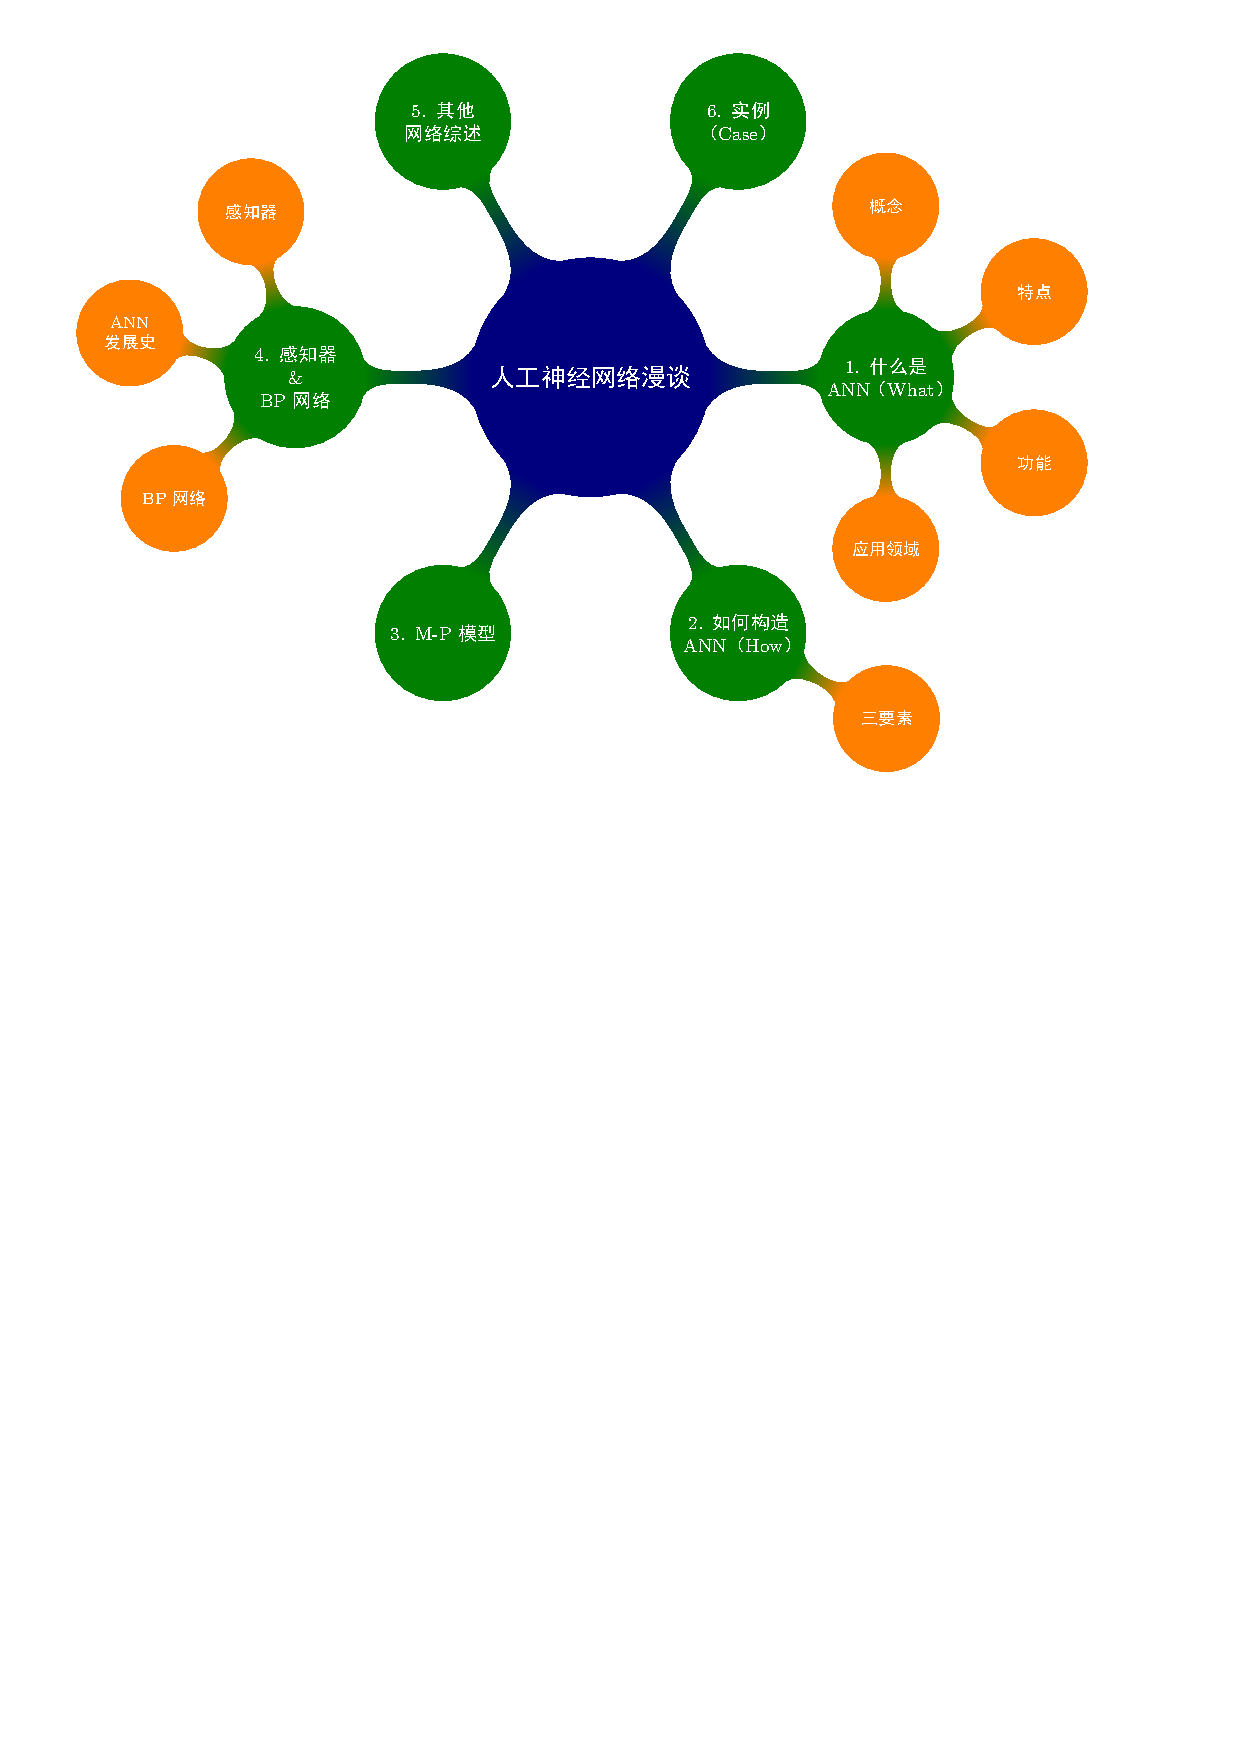
\includegraphics[width=\textwidth]{mindmap/map1.pdf}
  \end{figure}
\end{frame}

\section{什么是ANN}
\label{sec:what}

\begin{frame}{什么是人工神经网络?}
  \vspace{-1em}
  \begin{figure}
    \centering
    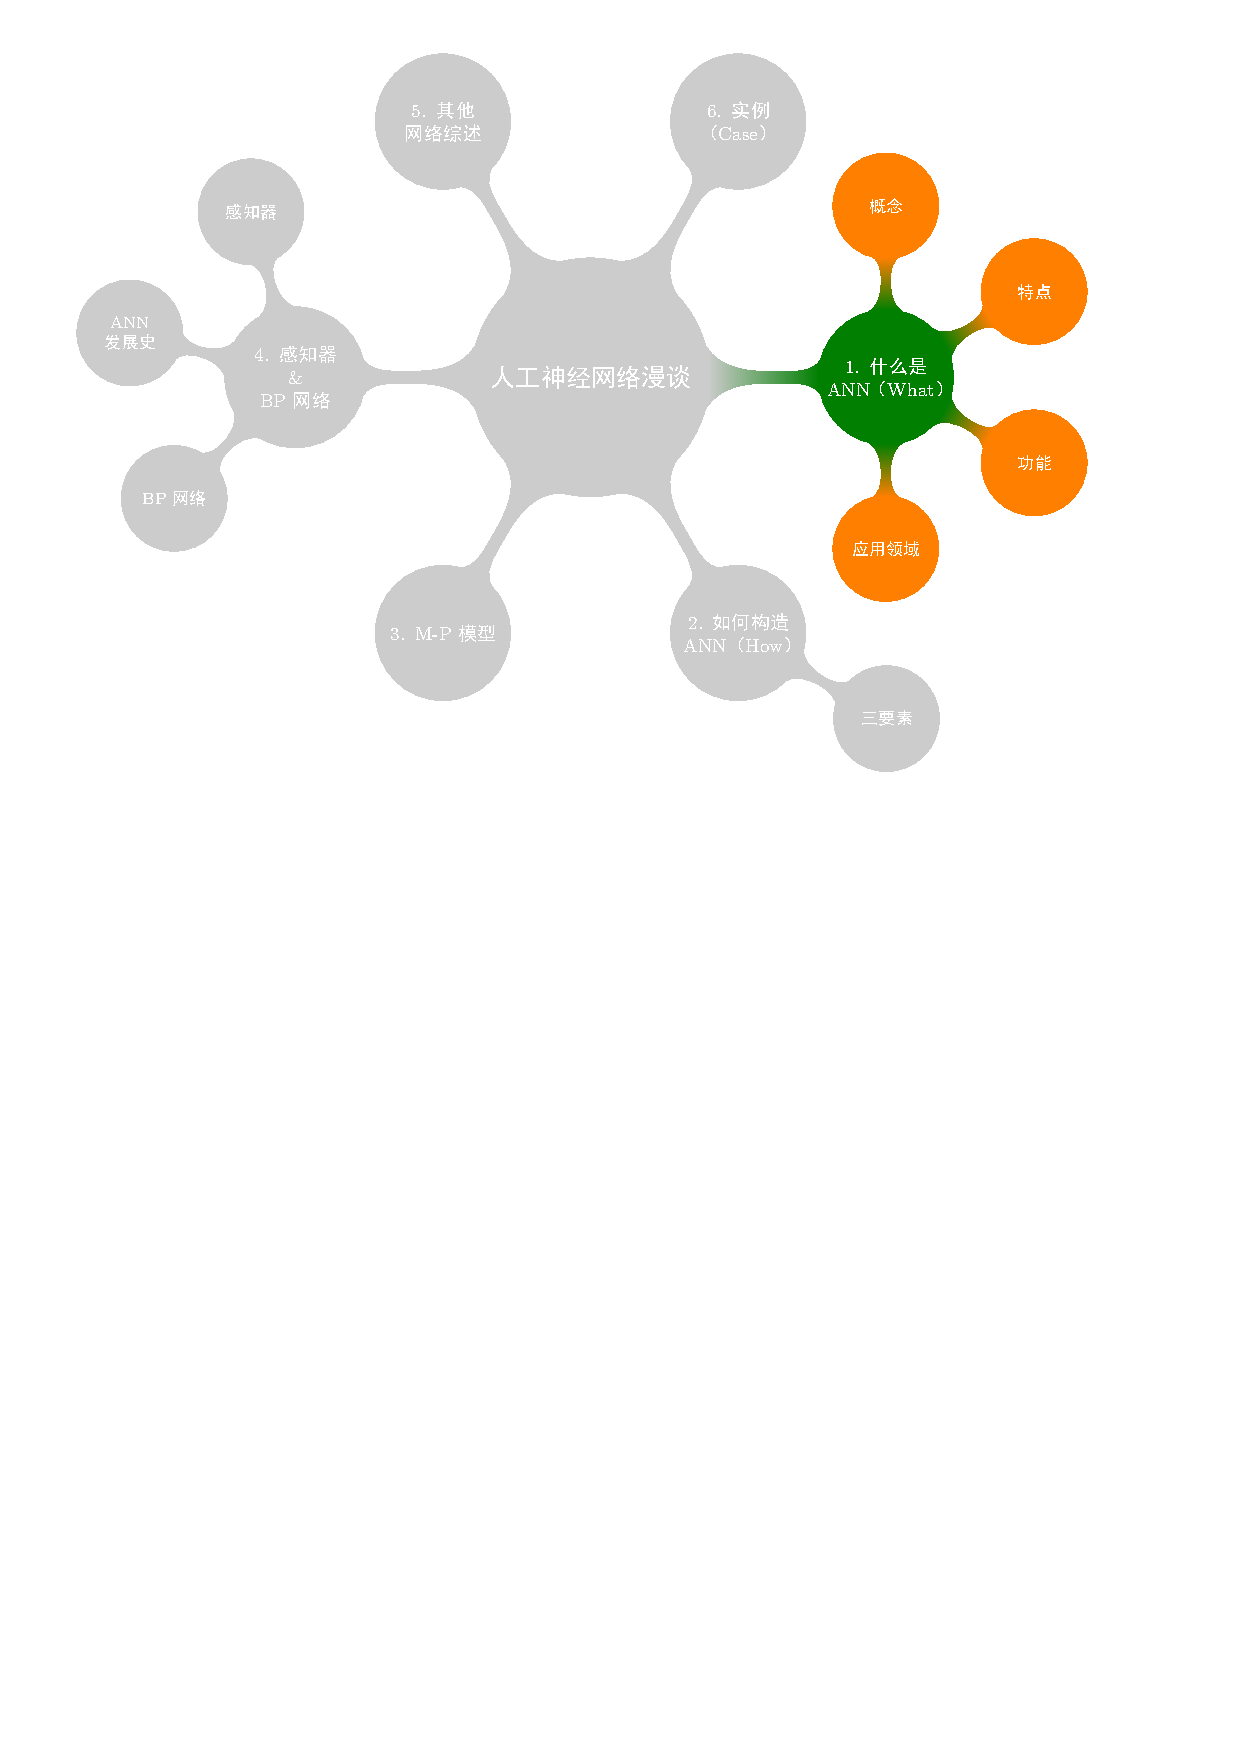
\includegraphics[width=\textwidth]{mindmap/map2.pdf}
  \end{figure}
\end{frame}

\subsection{人脑 V.S. 电脑}

\begin{frame}
  现代计算机的计算速度是人脑的几百万倍
  \begin{columns}
    \column{0.6\textwidth}
      加里 · 卡斯帕罗夫 \alert{V.S.} 超级计算机``深蓝''。
      \begin{itemize}
      \item 1996 4:2 卡斯帕罗夫胜
      \item 1997 2.5:3.5 ``深蓝''胜
      \end{itemize}

      \href{http://www.xqbase.com/computer/manvscomputer.htm}{\beamergotobutton{经典人机大战}}

      \column{0.4\textwidth}
        \centering
        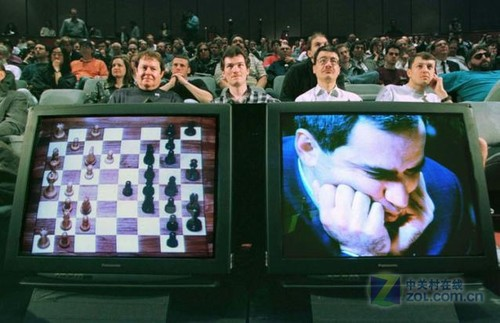
\includegraphics[width=\textwidth]{fig17.jpg}\\
        \vspace{1em}
        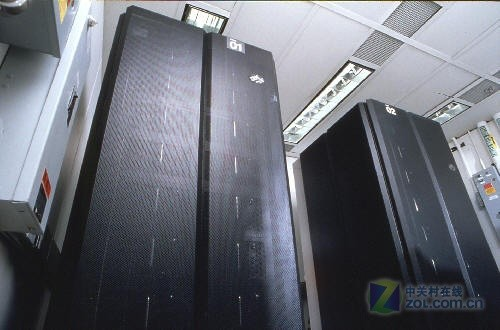
\includegraphics[width=\textwidth]{fig18.jpg}
  \end{columns}
\end{frame}

\begin{frame}
  然而对于一些问题,计算机却一直不如人类聪明
  \begin{itemize}
  \item 辨认人脸
  \item 开车
  \item 打篮球
  \item \ldots
  \end{itemize}
  \pause
  \begin{alertblock}{}
    只可意会,不可言传!
  \end{alertblock}
\end{frame}

\begin{frame}{人脑与电脑的机制区别}
    \pause
    人脑: 神经网络
    \pause
    \begin{itemize}[<+->]
    \item 规模庞大、结构精细的\alert{神经网络} $1.4\times 10^{11}$个神经细胞
    \item 处理的信息:\alert{模拟量}和离散脉冲
    \item 处理方式:\alert{并行}
    \item 擅长\alert{联想、创造}
    \end{itemize}
    \pause
    电脑: 冯 · 诺依曼 方式
    \pause
    \begin{itemize}[<+->]
    \item 存储器和处理器相互\alert{独立}
    \item 处理的信息:\alert{离散}的二进制数和二值逻辑形式
    \item 处理方式:\alert{串行}(取址、译码、执行、存储)
    \item 只擅长\alert{数值和逻辑运算}
    \end{itemize}
\end{frame}

\subsection{概念}
\label{sec:define}

\begin{frame}{什么是人工神经网络}
  \begin{columns}
    \column{.6\textwidth}
    \begin{itemize}
    \item 在对人脑神经网络的基本认识上,用数理方法从信息处理的角度对人脑神经网络进行\alert{抽象},并建立某种\alert{简化模型}。
    \item 不是人脑生物神经网络的真实写照,而只是对它的\alert{简化、抽象与模拟}。
    \item 旨在\alert{模仿}人脑结构及其功能的信息处理系统。
    \end{itemize}
    \column{.4\textwidth}
    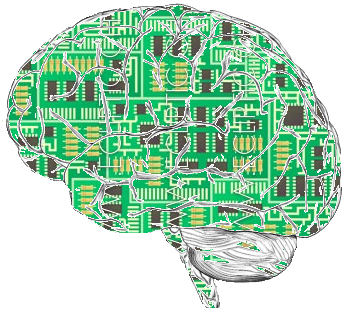
\includegraphics[width=\textwidth]{fig16.png}
  \end{columns}
\end{frame}

\subsection{特点和功能}
\label{sec:feature}

\begin{frame}{基本特点}
  \begin{center}
  \begin{tabular}{c|c|c}
    \hline 
    结构特点 & 性能特点 & 能力特征 \\
    \hline \hline
    \begin{tabular}{l}
      信息处理的并行性 \\
      信息存储的分布性 \\
      信息处理单元的互连性 \\
      结构的可塑性
    \end{tabular}
    &
    \begin{tabular}{l}
      高度的非线性 \\
      良好的容错性 \\
      计算的非精确性 
    \end{tabular}
    &
    \begin{tabular}{l}
      自学习\\
      自组织\\
      自适应性\\
    \end{tabular}
    \\
    \hline
  \end{tabular}
\end{center}
\end{frame}

\begin{frame}{基本功能}
  \begin{itemize}[<+->]
  \item 联想记忆
    \begin{itemize}
    \item 自联想记忆
    \item 异联想记忆
    \end{itemize}
  \item 非线性映射
  \item 分类与识别
  \item 优化计算
  \item 知识处理    
  \end{itemize}
\end{frame}

\subsection{应用领域}
\label{sec:apparea}

\begin{frame}{应用领域}
  \setlength\parindent{2em}
  神经网络学习方法对于逼近实数值、离散值或向量值的目标函
  数提供了一种健壮性很强的方法。对于某些类型的问题,如学习解释复杂的现实
  世界中的传感器数据,人工神经网络是目前知道的最有效的学习方法。

  \begin{center}
  \begin{tabular}{l|l}
    \hline 
    领域 & 应用举例 \\
    \hline \hline
    \\
    信息处理领域&信号处理、模式识别、数据压缩\\
    自动化领域&系统辨识、自动控制、智能检测\\
    工程领域&汽车工程、军事工程、化学工程、水利工程\\
    医学领域&检测数据分析、生物活性研究、医学专家系统\\
    经济领域&预测评估、信贷分析\\
    \ldots & \ldots \\
    \hline
  \end{tabular}
\end{center}
\end{frame}

\section{如何设计ANN}
\label{sec:how}

\subsection{问题}

\begin{frame}{如何设计ANN?}
  \vspace{-1em}
  \begin{figure}
    \centering
    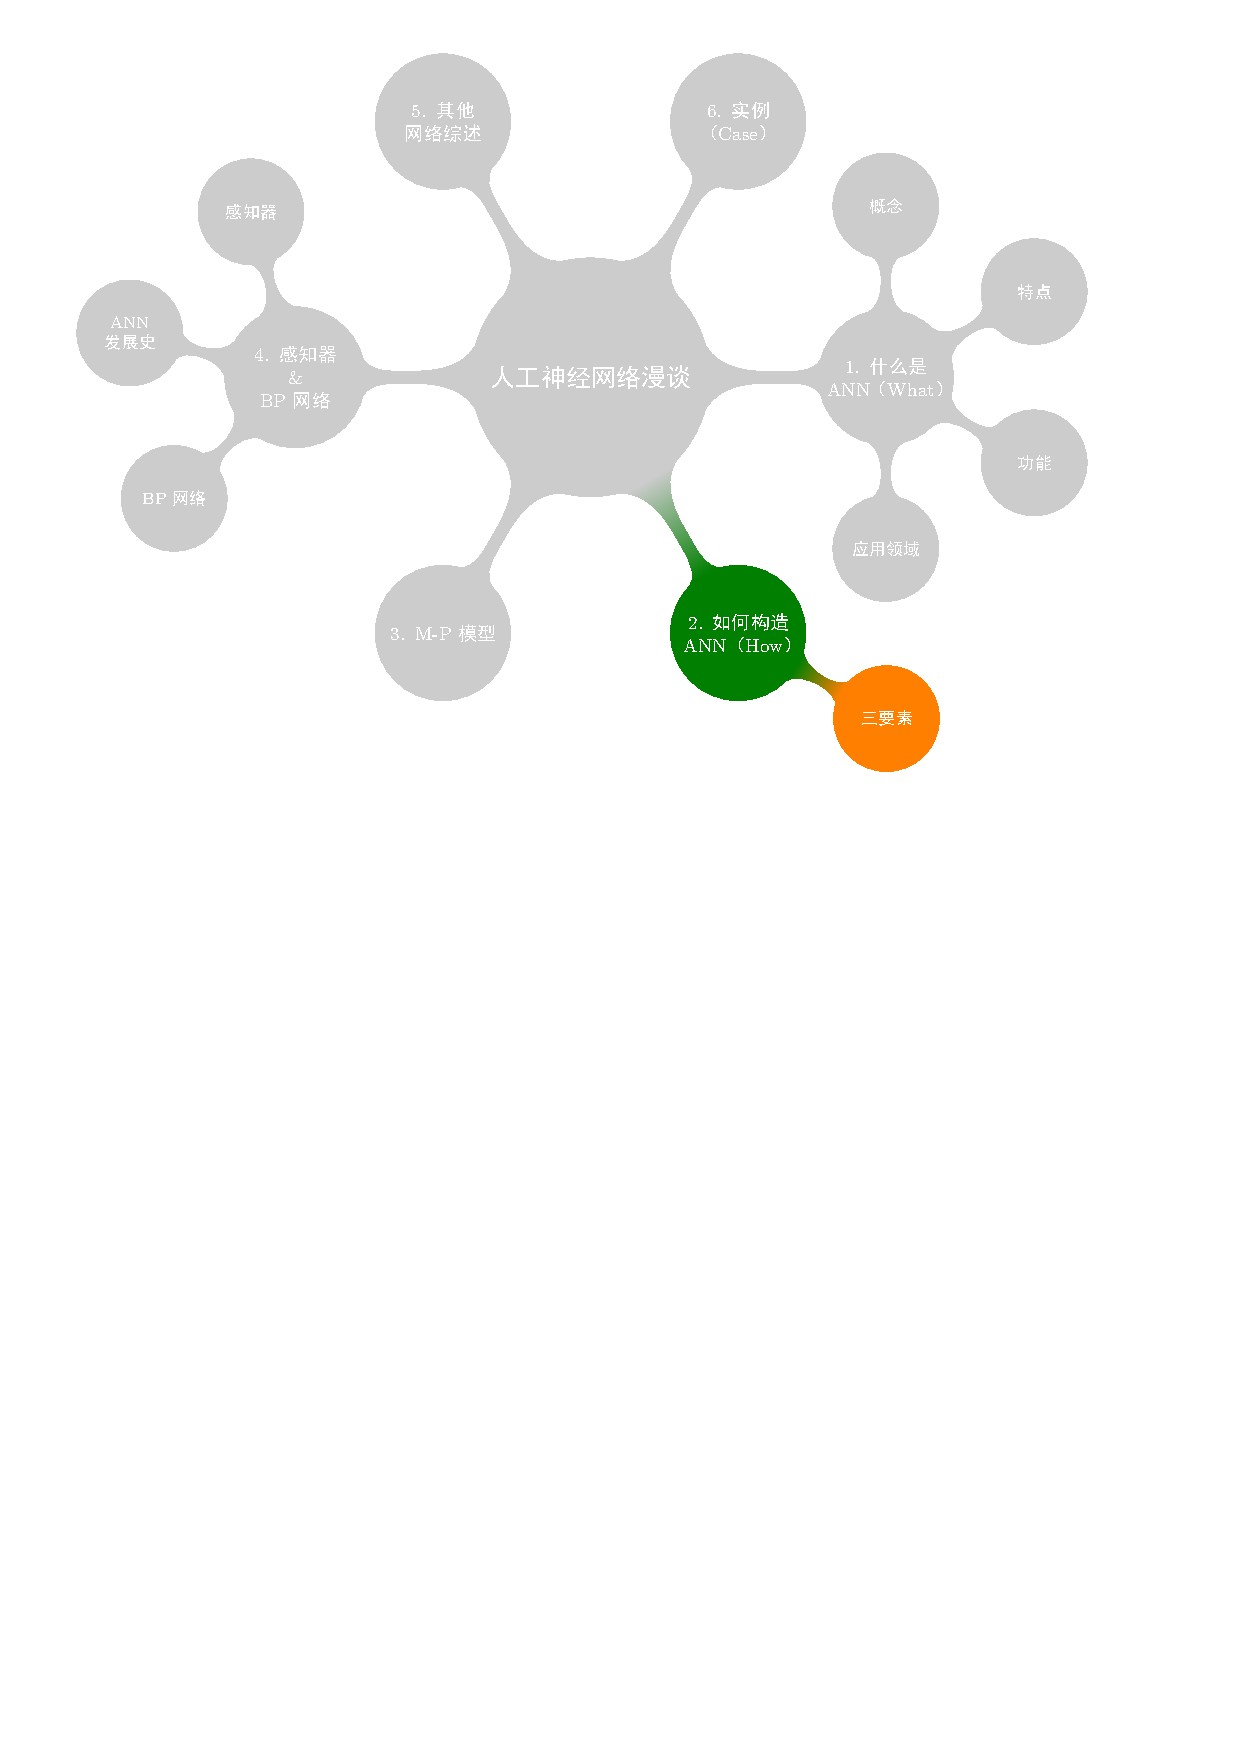
\includegraphics[width=\textwidth]{mindmap/map3.pdf}
  \end{figure}
\end{frame}

\begin{frame}{如何设计ANN?}
  \begin{enumerate}
  \item 构成神经网络的\alert{最小单位}是什么?
  \item 这些小单位\alert{怎么构造}成神经网络?
    \begin{itemize}
    \item 网络拓扑结构
    \end{itemize}
  \item 神经元之间如何进行\alert{信息传递}?
    \begin{itemize}
    \item 传递函数
    \end{itemize}
  \item 怎么\alert{训练}这个神经网络使它学会我们要的某些本领?
    \begin{itemize}
    \item 训练算法,或者叫学习规则(最终目的就是获得适用的权值)
    \end{itemize}
  \end{enumerate}
\end{frame}

\subsection{ANN三要素}

\begin{frame}{ANN三要素}
  \begin{figure}
    \centering
    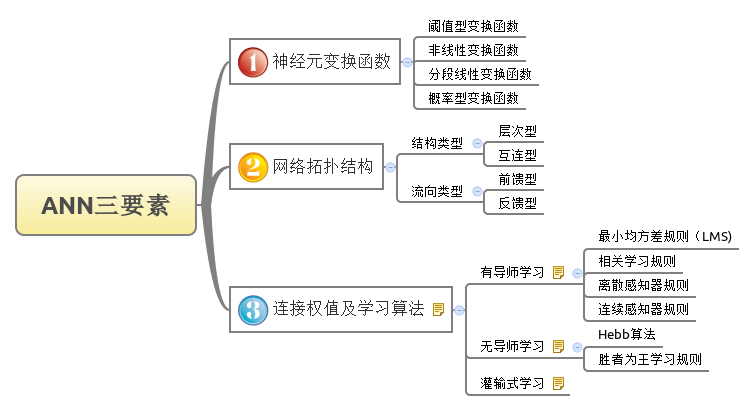
\includegraphics[width=0.9\textwidth]{fig19.png}
    \vspace{-1em}
    \caption{ANN三要素}
    \label{fig:3elements}
  \end{figure}
\end{frame}

\section{M-P模型}
\label{sec:mp}

\begin{frame}{M-P模型}
  \vspace{-1em}
  \begin{figure}
    \centering
    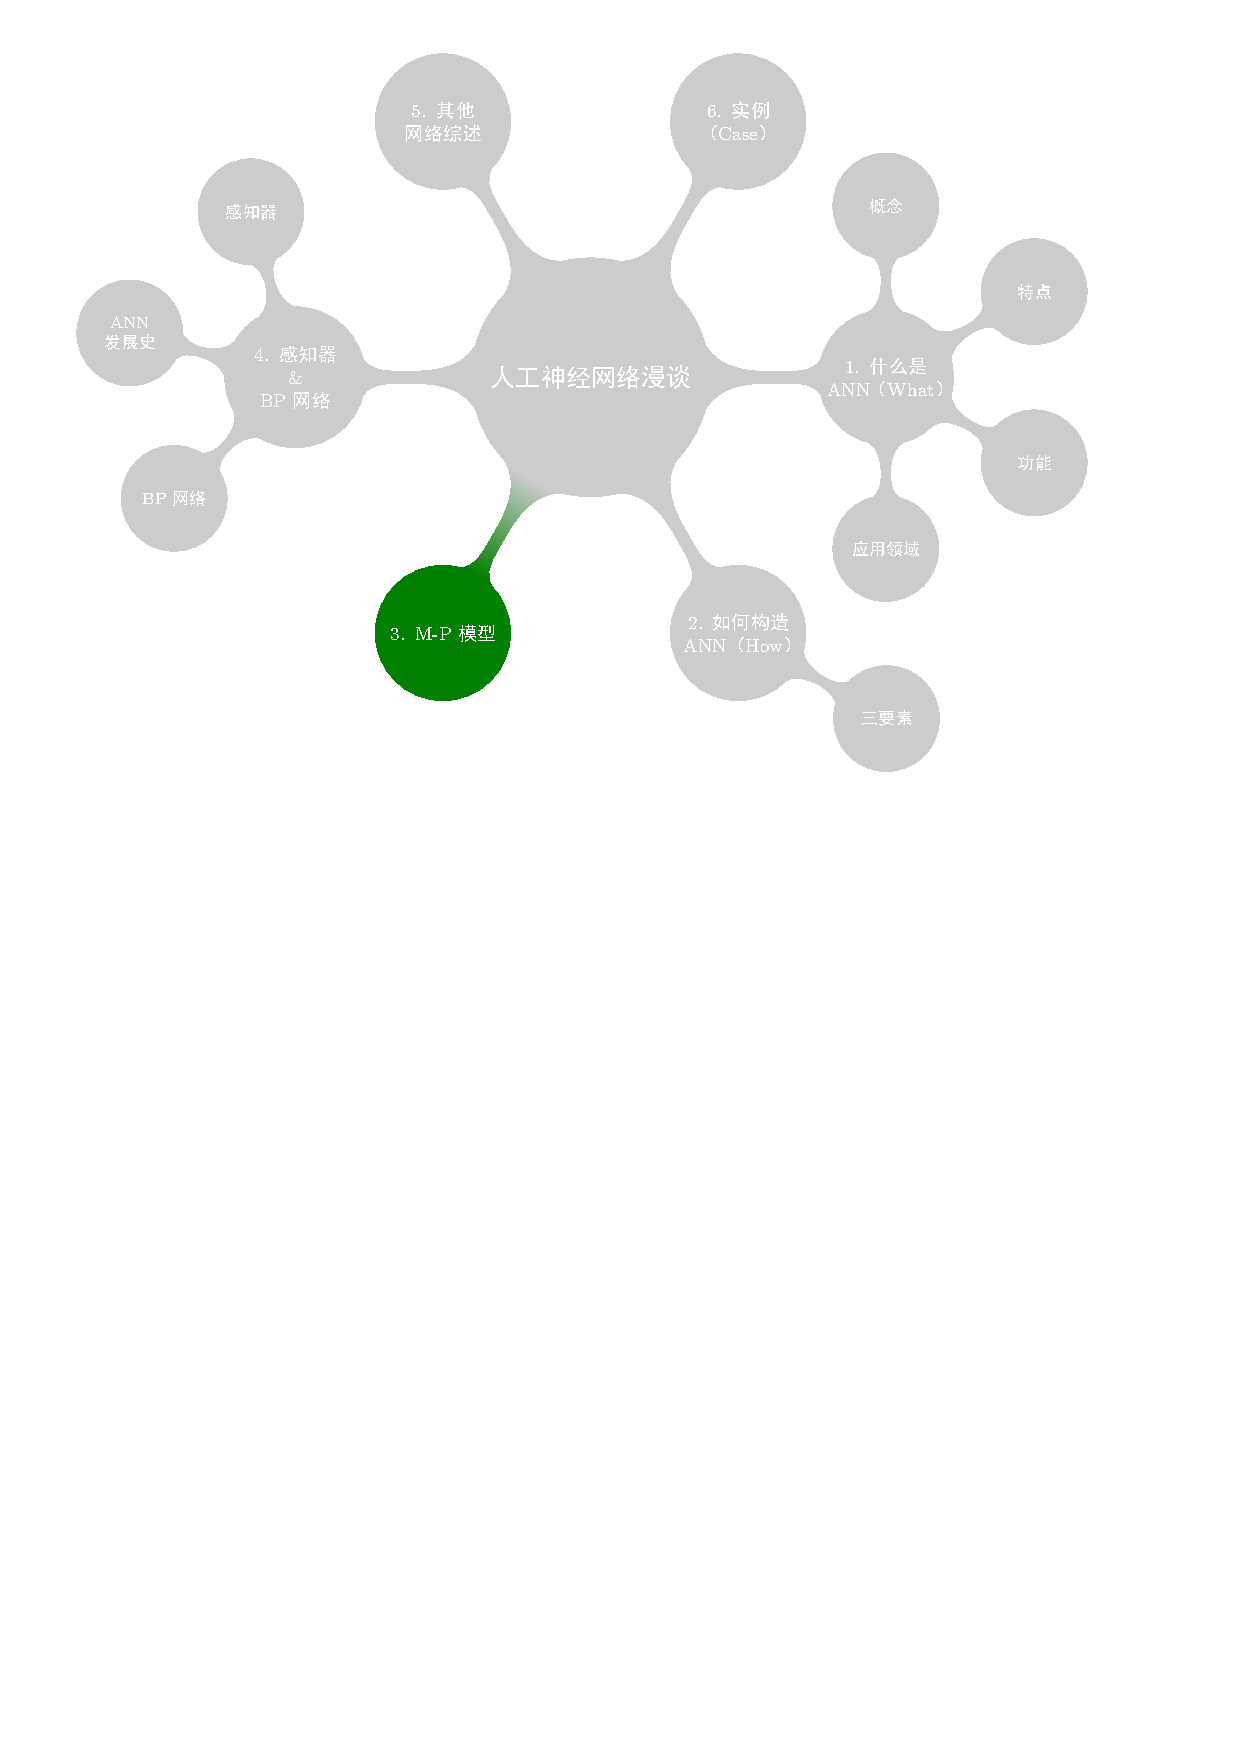
\includegraphics[width=\textwidth]{mindmap/map4.pdf}
  \end{figure}
\end{frame}

\begin{frame}{M-P模型}
  从最简单开始\pozhehao M-P模型
  \begin{itemize}
  \item M-P模型就是\alert{对一个生物神经元的建模}
  \item 它是心理学家W.McCulloch \& 数学家W.Pitts 于1943年提出的的模型
    (\alert{McCulloch-Pitts})
  \end{itemize}
  \begin{columns}
    \column{.5\textwidth}
    \begin{figure}
      \centering
      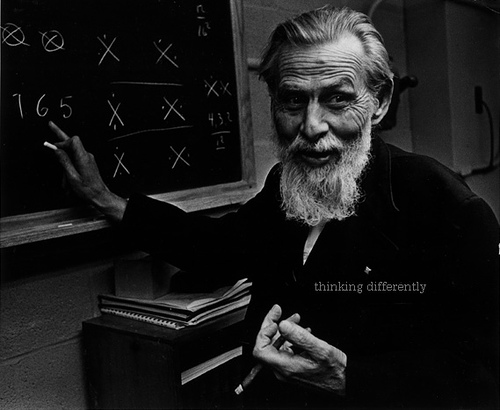
\includegraphics[height=.5\textheight]{fig22.jpg}
      \caption{Warren S. McCulloch}
      \label{fig:mcculloch}
    \end{figure}
    \column{.5\textwidth}
    \begin{figure}
      \centering
      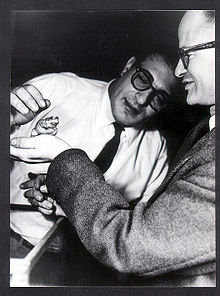
\includegraphics[height=.5\textheight]{fig23.jpg}
      \caption{Walter Pitts}
      \label{fig:mcculloch}
    \end{figure}
  \end{columns}
\end{frame}

\subsection{生物神经元}

\begin{frame}{生物神经元的结构}
  \setlength\parindent{2em}
  在谈M-P模型的内容之前,我们先得了解一下人脑中的神经元的结构,然后再研究M-P对人脑的神经元是如何建模的。
  \begin{itemize}
  \item 神经元是脑组织的基本单元
  \item 人脑中大约包含$1.4\times 10^{11}$个神经元
  \item 每个神经元与大约$10^3\sim 10^5$个其他神经元相连接
  \end{itemize}
\end{frame}

\begin{frame}{生物神经元的结构}
  Figure \ref{fig:cell}是一张生物神经元的简化示意图。

  \begin{figure}
    \centering
    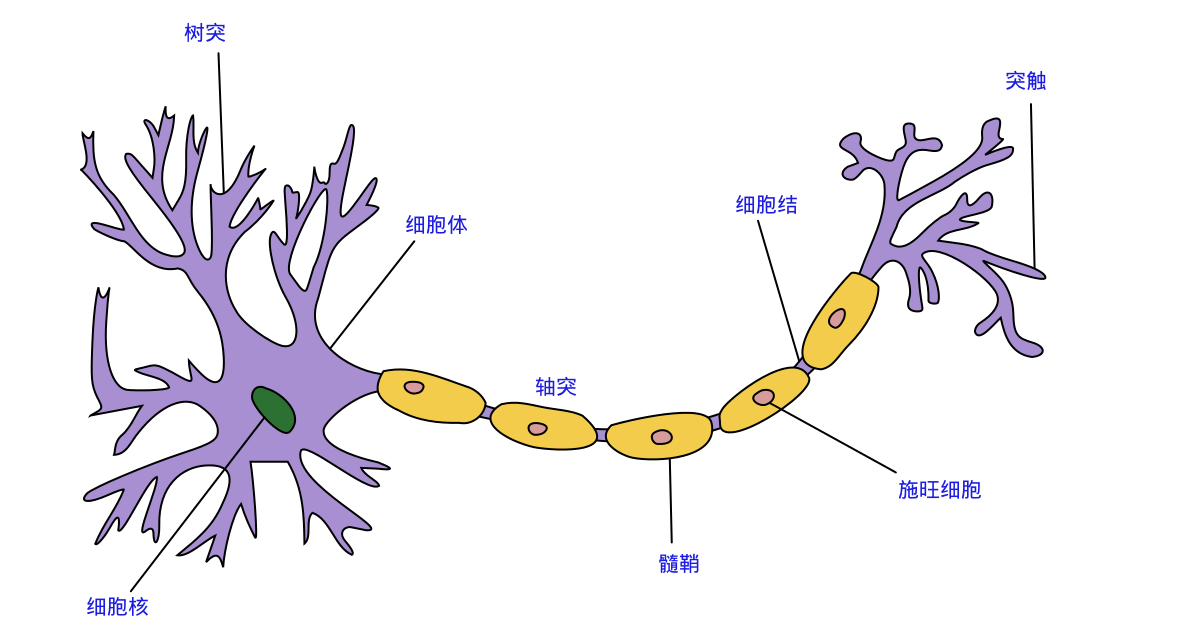
\includegraphics[width=.9\textwidth]{fig28.png}
    \vspace{-1em}
    \caption{生物神经元简化示意图}
    \label{fig:cell}
  \end{figure}
\end{frame}

\begin{frame}{生物神经元的结构}
  \small
  神经元在结构上由\alert{细胞体}、\alert{树突}、\alert{轴突}和\alert{突触}4部分组成。
  \begin{enumerate}
  \item 细胞体\\
    神经元的主体,由\alert{细胞核}、\alert{细胞质}和\alert{细胞膜}3部分组成。细胞体的外部是细胞膜,将膜内外细胞液分开。由于细胞膜对细胞液中的不同离子具有不同的通透性,这使得膜内外存在着离子浓度差,从而出现内负外正的静息电位。这种电位差称为\alert{膜电位}。
  \item 树突\\
    从细胞体向外延伸出许多突起的神经纤维。负责接收来自其他神经元的输入信号,相当于细胞体的\alert{输入端(input)}。
  \item 轴突\\
    由细胞体伸出的最长的一条突起称为轴突。轴突比树突长而细。轴突也叫神经纤维,末端处有很多细的分支称为神经末梢,每一条神经末梢可以向四面八方传出信号,相当于细胞体的\alert{输出端(output)}。
  \item 突触\\
    一个神经元通过其轴突的神经末梢和和另一个神经元的细胞体或树突进行\alert{通信连接},称为突触。
  \end{enumerate}
\end{frame}


\begin{frame}{生物神经元的结构}
  \setlength\parindent{2em}
  
  突触使神经细胞的膜电位发生变化,且电位的变化是可以\alert{累加}的,单个神经元可
  以与多达上千个其他神经元的轴突末梢形成突触连接,接受从各个轴突传来的\alert{脉
    冲}输入。这些输入可到达神经元的不同部位,输入部位不同,对神经元影响
  的\alert{权重}也不同。输入部位不同,该神经细胞\alert{膜电位}是它所有突触产生
  的\alert{电位总和},当该神经细胞的膜电位升高到超过一个\alert{阈值}时,就会产生
  一个\alert{脉冲},从而总和的膜电位直接影响该神经细胞兴奋发放的脉冲数。

  神经元的信息是宽度和幅度都相同的\alert{脉冲串},若某个神经细胞兴奋,其轴突输出
  的脉冲串的频率就高;若某个神经细胞抑制,其轴突输出的脉冲串的频率就低,甚至无脉
  冲输出。因此,突触可以分为\alert{兴奋性}和\alert{抑制性}两种,兴奋性的突触可能
  引起下一个神经细胞兴奋,抑制性的突触使下一个神经细胞抑制。脉冲的传递是\alert{正
    向}的,不允许逆向传播。另外,突触传递信息需要一定的\alert{延迟}。
\end{frame}


\begin{frame}{比喻\Rmnum{1}:水桶模型}
  
  \begin{columns}
    \column{.5\textwidth}
    \begin{figure}
      \centering
      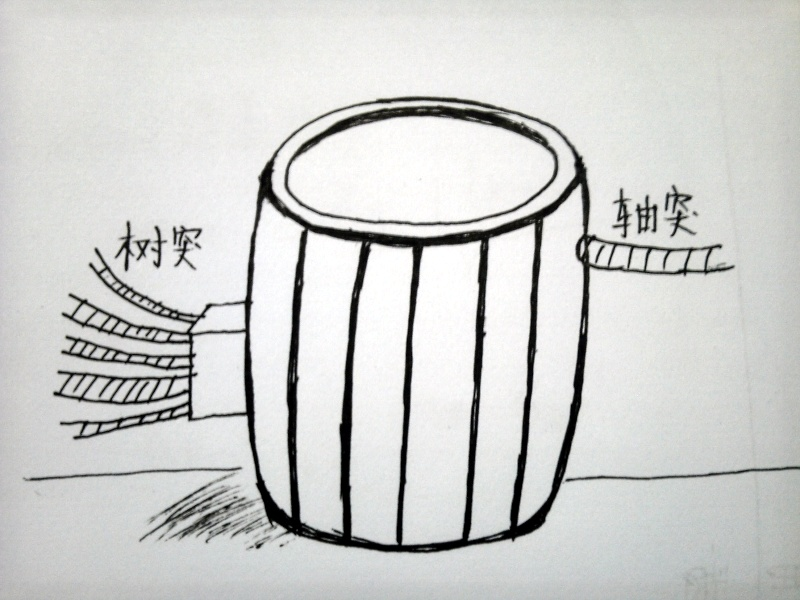
\includegraphics[width=\textwidth]{fig29.jpg}
      \caption{水桶与神经元}
      \label{fig:barrel}
    \end{figure}
    \column{.5\textwidth}

    \small

    \setlength\parindent{2em}
    
    我的一个比喻:可以把一个神经元想象成一个水桶,这个水桶侧边接着很多条水管(\alert{神经末
      梢}),水管既可以将桶里的水输出去(\alert{抑制性}),也可以将其他水桶的水输
    进来(\alert{兴奋性})。当桶里的水达到一个高度(\alert{阈值})时,就会通过另
    一条管子(\alert{轴突})将水输送出去。由于水管的粗细不同,对桶里的水的影响程
    度(\alert{权重})也不同。水管对水桶里的水位的改变(\alert{膜电位})自然就是
    这些水管输水量的累加。    
    
  \end{columns}
\end{frame}

\begin{frame}{比喻\Rmnum{2}:选餐馆}
  我该去哪间餐馆吃饭?
  
  \begin{center}
    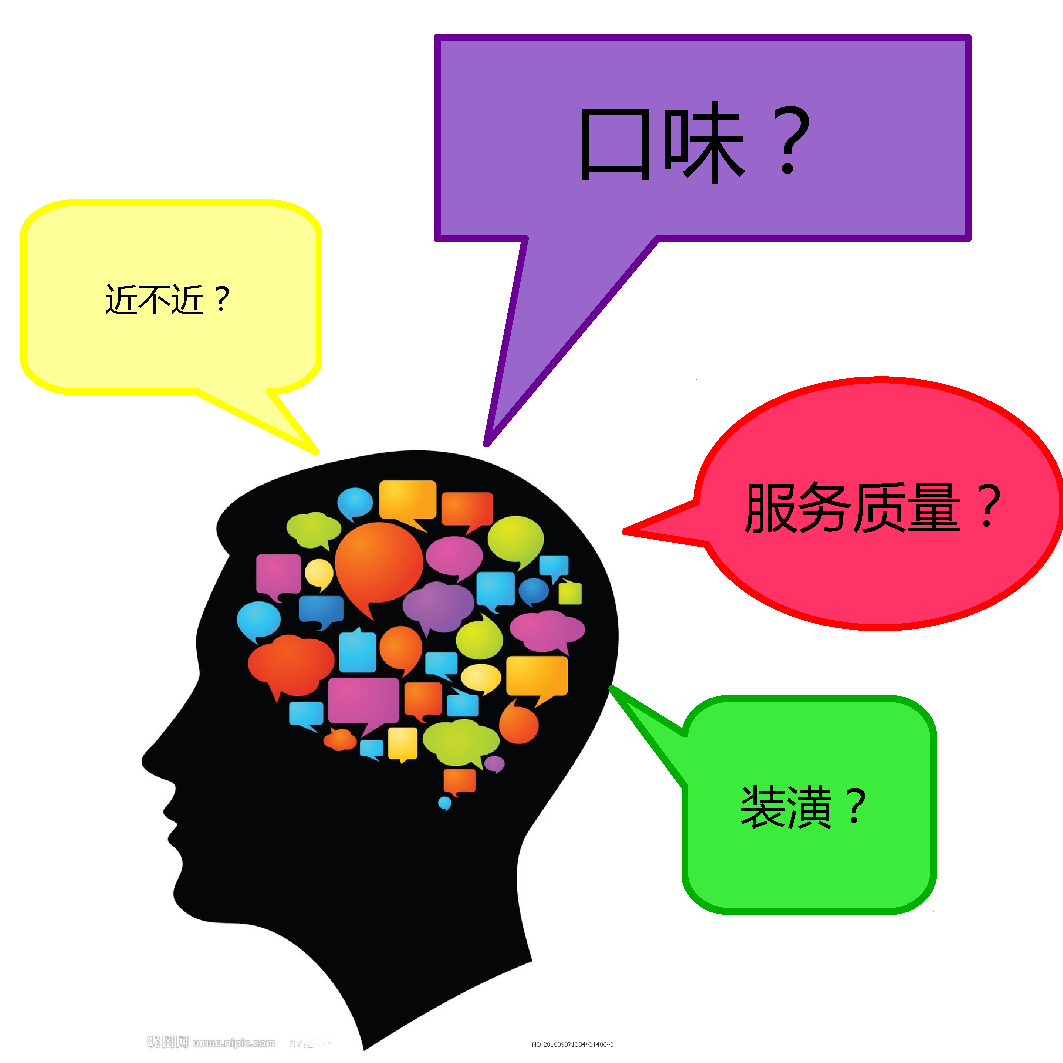
\includegraphics[width=.5\textwidth]{fig30.pdf}
  \end{center}
\end{frame}

\subsection{M-P模型}

\begin{frame}{M-P模型}
  \setlength\parindent{2em}
  
  按照生物神经元,我们建立 \alert{M-P模型}。为了使得建模更加简单,以便于进行形式化
  表达,我们忽略时间整合作用、不应期等复杂因素,并把神经元的突触时延和强度当成常
  数。Figure \ref{fig:m-p}就是一个M-P模型的示意图。

  \begin{figure}
    \centering
    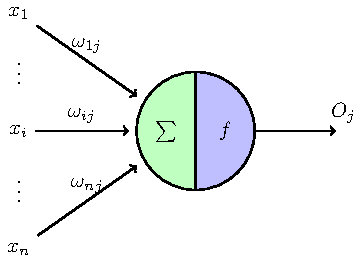
\includegraphics[width=.5\textwidth]{fig41.pdf}
    \caption{M-P模型}
    \label{fig:m-p}
  \end{figure}
  
\end{frame}

\begin{frame}{M-P模型}
  参照生物神经元,我们定义以下几个重要的参数:
  \vspace{-1em}
  \begin{table}
    \begin{center}
      \small
      \caption{M-P模型几个重要的参数}
      \vspace{-1em}      
      \label{tab:bvsmp}
      \begin{tabular}{cccccccc}
        \hline
        生物神经元 & 神经元 & 输入信号 & 权值 & 输出 & 总和 & 膜电位 & 阈值\\
        M-P模型   & $j$ & $X_i$ & $\omega_{ij}$ & $O_j$ & $\sum$ &
        $\sum_{i=1}^n\omega_{ij}X_i(t)$ & $T_j$\\
        \hline
      \end{tabular}
    \end{center}
    \flushleft
    
    对于某一个神经元\(j\),它可能接受同时接受了许多个输入信号,用\(\chi_{i}\)表示,
    前面说过,由于生物神经元具有不同的突触性质和突触强度(水管粗细不同),所以对神
    经元的影响不同,我们用权值\(\omega_{ij}\)来表示,其正负模拟了生物神经元中突出
    的兴奋和抑制(进水和出水),其大小则代表了突出的不同连接强度。由于累加性,我们
    对全部输入信号进行累加整合,相当于生物神经元中的膜电位(水的变化总量),其值就
    为
    % \vspace{-1em}
    \begin{equation}
      \label{eq:net}
      net'_j(t)=\sum_{i=1}^n\omega_{ij}\chi_{i}(t)    
    \end{equation}

  \end{table}
\end{frame}

\begin{frame}{M-P模型}
  神经元激活与否(外接专用水管流出与否)取决于某一阈值电平(水位高度),即只有当
  其输入总和超过阈值Tj时,神经元才被激活而发放脉冲,否则神经元不会发生输出信号。
  整个过程可以用下面这个函数来表示:
  
  \begin{equation}
  \label{eq:mp}
    o_{j}(t) = f{[\sum_{i=1}^n\omega_{ij}\chi_{i}(t)]-T_{j}}
  \end{equation}
\end{frame}

\begin{frame}{}
  如果\(\chi_0 = -1\),\(\omega_{0j} = T_j\),则有\(-T_j = \chi_0\omega_{0j}\)。
  
  因此公式(\ref{eq:net})和(\ref{eq:mp})还可以简化成公式(\ref{eq:sim1})和(\ref{eq:sim2})的形式:

  \begin{equation}
    \label{eq:sim1}
    net'_j = W_j^TX
  \end{equation}

  \begin{equation}
    \label{eq:sim2}
    o_j = f(net_j) = f(W_j^TX)
  \end{equation}
\end{frame}


\begin{frame}{M-P模型的特点}
  由此我们可以得到总结出M-P模型的6个特点:
  \begin{enumerate}
  \item 每个神经元都是一个\alert{多输入单输出}的信息处理单元;
  \item 神经元输入分\alert{兴奋性输入}和\alert{抑制性}输入两种类型;
  \item 神经元具有\alert{空间整合特性}和\alert{阈值特性};
  \item 神经元输入与输出间有固定的\alert{时滞},主要取决于突触延搁;
  \item \alert{忽略}时间整合作用和不应期;
  \item 神经元本身是\alert{非时变}的,即其突触时延和突触强度均为常数。
  \end{enumerate}
\end{frame}

\section{感知器 \& BP网络}
\label{sec:perceptron}

\begin{frame}{感知器 \& BP网络}
    \vspace{-1em}
  \begin{figure}
    \centering
    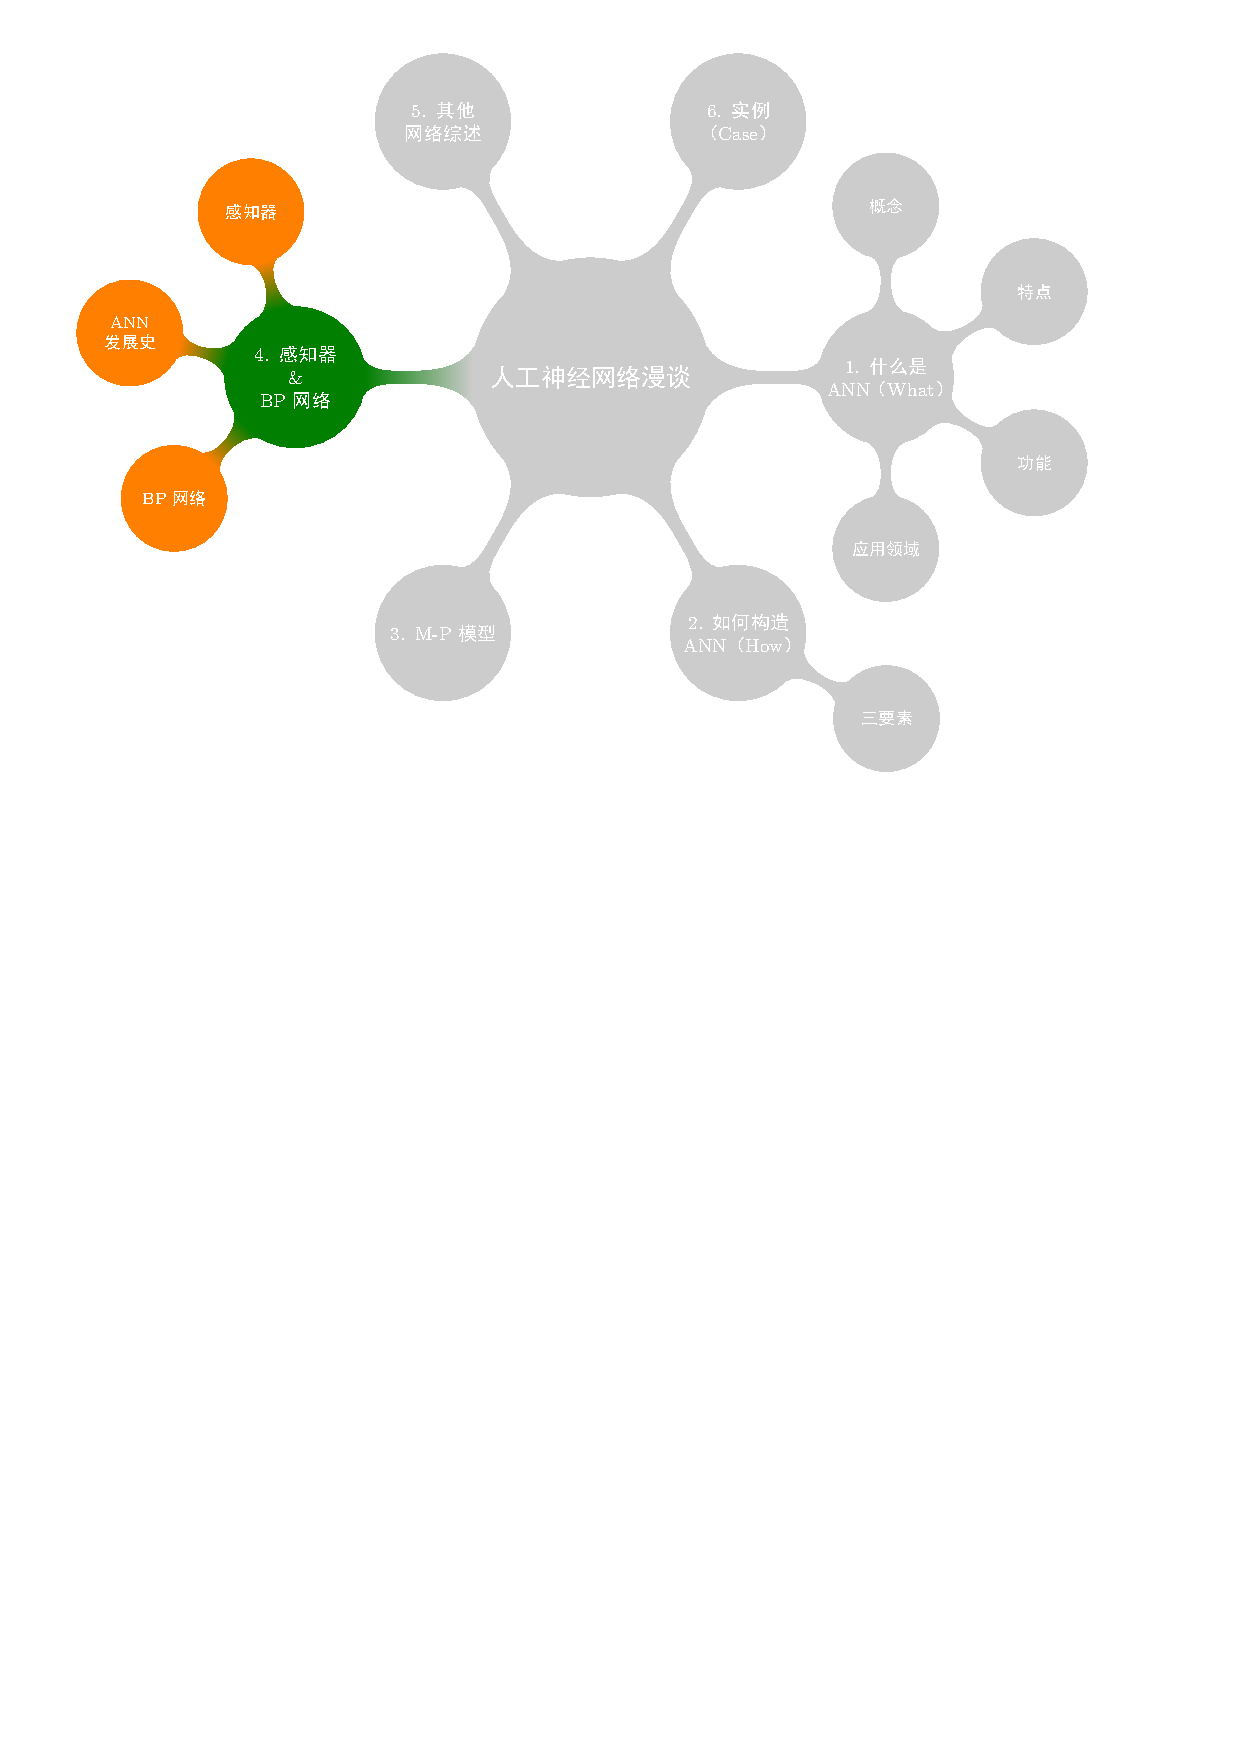
\includegraphics[width=\textwidth]{mindmap/map5.pdf}
  \end{figure}
\end{frame}

\subsection{感知器}

\begin{frame}{什么是感知器}
  M-P模型只是对单个神经元的建模,还不足以模拟人脑神经系统的功能。由这些人工神经元
  构建出来的网络,才能够具有学习、联想、记忆和模式识别的能力。
  \begin{itemize}
  \item 怎么连?
  \item 信号怎么传递?
  \item 怎么训练?
  \end{itemize}
\end{frame}

\begin{frame}{最简单的神经网络结构\pozhehao 单层感知器}
  1958年,美国心理学家Frank Rosenblatt提出一种具有%
  \alert{单层计算单元}的神经网络,称为\alert{感知器}(Perceptron)。
  \begin{figure}
    \centering
    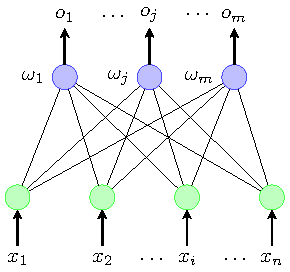
\includegraphics[width=0.5\textwidth]{fig02.pdf}
    \vspace{-1em}
    \caption{单层感知器拓扑结构}
    \label{single}
  \end{figure}
\end{frame}

\begin{frame}{单层感知器}
  \begin{itemize}
  \item
    输入加权和
    \begin{equation} net'_j=\sum_{i=1}^n\omega_{ij}\chi_i \end{equation}
  \item 学习规则:离散感知器学习规则(有导师学习)
  \item 传递函数:sgn函数\\
    \begin{equation}
      \label{eq:sgn}
      o_j=sgn(net'_j-T_j)=sgn(\sum_{i=0}^n\omega_ij\chi_i)=sgn(W_j^TX)
    \end{equation}
  \item 公式(\ref{eq:sgn})可以进一步表达为:
    \begin{equation}
      o_j=\left \{ \begin{aligned} 1 & ~~~ W_j^TX>0 \\ -1 & ~~~ W_j^TX<0 \end{aligned} \right.
    \end{equation}
  \end{itemize}
\end{frame}

\begin{frame}{风中之烛——单层感知器的局限性}
  
  \alert{单层感知器仅对线性问题具有分类能力}。

  ~
  
  线性问题:简单来讲,就是用一条直线可分的图形。比如:
  \begin{itemize}
  \item 逻辑``与''
  \item 逻辑``或''
  \end{itemize}
  我们可以用一条直线来分隔0和1。
\end{frame}

\begin{frame}{逻辑``与''的真值表及二维样本分类图}
  \begin{columns}
    \column{.5\textwidth}
    \begin{table}
      \centering
      \begin{tabular}[b] {lll}
        $x_1$ & $x_2$ & $y$ \\
        0 & 0 & 0\\
        0 & 1 & 0\\
        1 & 0 & 0\\
        1 & 1 & 1\\
      \end{tabular}
    \end{table}
    \column{.5\textwidth}
    \begin{figure}
      \centering
      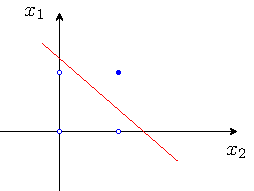
\includegraphics[width=\textwidth]{fig32.pdf}
      \caption{逻辑``与''的二维样本分类图}
      \label{fig:logicand}
    \end{figure}
  \end{columns}
\end{frame}

\begin{frame}{逻辑``或''的真值表及二维样本分类图}
  \begin{columns}
    \column{.5\textwidth}
    \begin{table}
      \centering
      \begin{tabular}[b]  {lll}
	$x_1$ & $x_2$ & $y$ \\
	0 & 0 & 0\\
	0 & 1 & 1\\
	1 & 0 & 1\\
	1 & 1 & 1\\
      \end{tabular}
    \end{table}
    \column{.5\textwidth}
    \begin{figure}
      \centering
      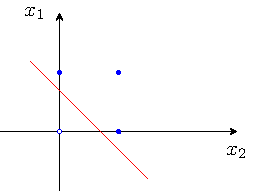
\includegraphics[width=\textwidth]{fig33.pdf}
      \caption{逻辑``或''的二维样本分类图}
      \label{fig:logicor}
    \end{figure}
  \end{columns}
\end{frame}

\begin{frame}
  为什么感知器就可以解决线性问题呢?这是由它的\alert{传递函数}决定的。这里以两个输入分
  量\(x_1\)和\(x_2\)组成的二维空间为例,此时节点\(j\)的输出为
  
  \[ o_j=\left \{ \begin{aligned} 1 & ~~~\omega_{1j}x_1+\omega_{2j}x_2-T_j>0 \\
      -1 & ~~~\omega_{1j}x_1+\omega _{2j}x_2-T_j<0 \end{aligned} \right. \]
  
  所以,方程
  \begin{equation}
    \label{eq:linear}
    \omega_{1j}x_1+\omega_{2j}x_2-T_j=0
  \end{equation}
  确定的直线就是二维输入样本空间上的一条分界线。
\end{frame}

\begin{frame}{``异或''的真值表及二维样本分类图}
  如果要让它来处理非线性的问题,单层感知器网就无能为力了。例如下面的“异或”,就无法用一条直线来分割开来,因此单层感知器网就没办法实现“异或”的功能。
  \begin{columns}
    \column{.5\textwidth}
    \begin{table}
      \centering
      \begin{tabular}[b] {lll}
        $x_1$ & $x_2$ & $y$ \\
	0 & 0 & 0\\
	0 & 1 & 1\\
	1 & 0 & 1\\
	1 & 1 & 0\\
      \end{tabular}
    \end{table}
    \column{.5\textwidth}
    \begin{figure}
      \centering
      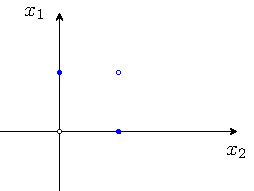
\includegraphics[width=\textwidth]{fig34.pdf}
      \caption{``异或''的二维样本分类图}
      \label{fig:logicxor}
    \end{figure}
  \end{columns}
\end{frame}

\subsection{多层感知器}
\label{sec:multilayer}

\begin{frame}{多层感知器}

  \setlength\parindent{2em}
  
  所谓多层感知器,就是在输入层和输出层之间加入隐层,,以形成能够将样本正确分类的
  凸域。多层感知器的拓扑结构如Figure\ref{fig:mullayer}所示。
  
  \centering
  \begin{figure}
    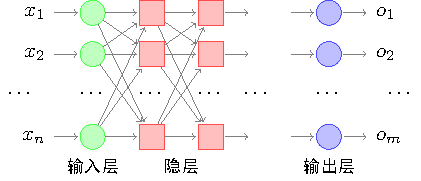
\includegraphics[width=0.8\textwidth]{fig04.pdf}
    \caption{多层感知器的拓扑结构}
    \label{fig:mullayer}    
  \end{figure}
\end{frame}

\begin{frame}{多层感知器}
  \begin{itemize}
  \item 我们可以比较一下单层感知器和多层感知器的分类能力:
  \end{itemize}
  \begin{table}
    \centering
    \caption{不同隐层数感知器的分类能力}
    \label{fig:different}
    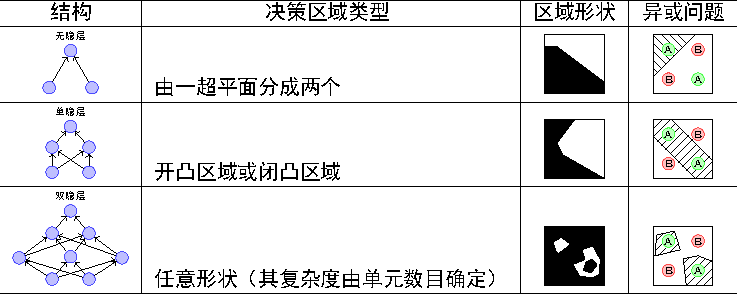
\includegraphics[width=\textwidth]{fig03.pdf}
  \end{table}
\end{frame}

\begin{frame}{心有余而力不足\pozhehao 多层感知器的瓶颈}
  Kolmogorov理论指出:\alert{双隐层感知器足以解决任何复杂的分类问题。}

  ~

  1966年Minsky和Papert《感知器》:\alert{多层感知器能够求解非线性问题,但对隐层神
    经元的学习规则尚无所知。}权值调整量取决于感知器期望输出与实际输出之差,
  即\begin{equation} \Delta W_j(t) = \eta[d_j-o_j(t)]X \end{equation}对于各隐层节
  点来说,不存在期望输出,因而该学习规则对隐层权值不适用。
\end{frame}



\begin{frame}{山重水复疑无路——ANN的低潮期}
  1966年,Minisky和Papert在他们的《感知器》一书中提出了上述的感知器的研究瓶颈,指
  出理论上还不能证明将感知器模型扩展到多层网络是有意义的。这在人工神经网络的历史
  上书写了极其灰暗的一章。
  \begin{figure}
    \centering
    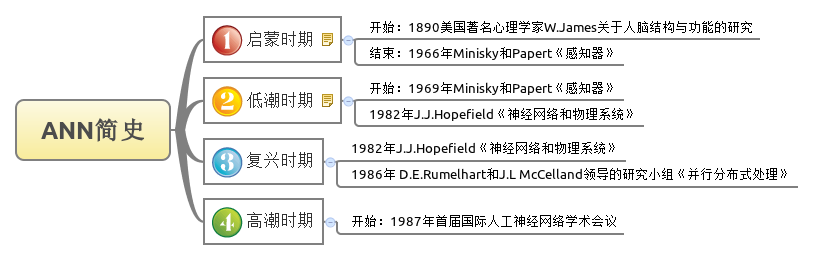
\includegraphics[width=\textwidth]{fig05.png}
    \caption{ANN发展史}
    \label{fig:history}
  \end{figure}
\end{frame}

\subsection{BP网络}

\begin{frame}{柳暗花明又一村——ANN研究的复苏和BP神经网络的诞生}
  尽管ANN的研究陷入了前所未有的低谷,但仍有为数不多的学者忍受住寂寞,坚持致力
  于ANN的研究。在长达10年的低潮时期之间,相继有一些开创性的研究成果被提出来,但还
  不足以激起人们对于ANN研究的热情。一直到上世纪80年代,两个璀璨的成果诞生
  了:1982年美国加州理工学院的物理学家John J.Hopfield博士的Hopfield网络和David
  E.Rumelhart以及James L.McCelland研究小组发表的《并行分布式处理》。这两个成果重
  新激起了人们对ANN的研究兴趣,使人们对模仿脑信息处理的智能计算机的研究重新充满了
  希望。
\end{frame}

\begin{frame}{BP网络}
  \begin{itemize}
  \item
    1986年,Rumerhart和McCelland《平行分布式处理》对具有非线性连续变换函%
    数的多层感知器的\alert{误差反传(Error Back Propagation, BP)%
      算法}进行了详尽的分析,实现了Minsky关于多层网络的设想。
  \item
    由于多层感知器网络的训练经常采用误差反向传播算法,人们也常把多层感知器直接称为BP网。
  \end{itemize}
\end{frame}

\begin{frame}{误差反传算法}
  \begin{itemize}
  \item
    Back Propagation was created by \alert{generalizing} the \alert{
      Widrow-Hoff} learning rule to \alert{multiple-layer} networks and
    \alert{nonlinear} differentiable transfer function.
  \item
    误差反传算法 (BP算法、$\delta$算法)
    \begin{itemize}
    \item 信号的正向传播
    \item 误差的反向传播
    \end{itemize}
  \item
    BP算法的基本思想是,学习过程由信号的正向传播与误差的反向传播两个过程组成。
  \end{itemize}
\end{frame}


\begin{frame}{误差反传算法}
  \begin{block}{信号的正向传播}
    \begin{itemize}
    \item
      正向传播时,输入样本从输入层传入,经各隐层逐层处理后,传向输出层。
    \item
      若输出层的实际输出与期望的输出(教师信号)不符,则转入误差的反向传播阶段。
    \end{itemize}
  \end{block}
  \begin{block}{误差的反向传播}
    \begin{itemize}
    \item 将输出以某种形式通过隐层向输入层逐层反传,并将误差分摊给各层的所有单元,从而获得%
      各层单元的误差信号,此误差信号即作为修正各单元权值的依据。
    \end{itemize}
  \end{block}
\end{frame}

\begin{frame}{BP算法的信号流向}
  \begin{figure}
    \begin{center}
      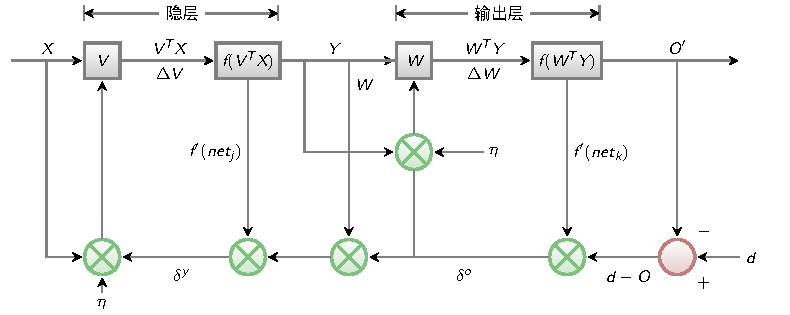
\includegraphics[width=\textwidth]{fig06.pdf}
    \end{center}
    \caption{BP算法的信号流向图}
    \label{signal}
  \end{figure}
\end{frame}

\begin{frame}{BP网络的结构}
  \begin{itemize}
  \item \alert{多层感知器} [figure \alert{\ref{fig:mullayer}}],其中单隐层网络(三层感知器)的应用最为普遍。
  \item 三层:输入层、隐层、输出层。
  \end{itemize}
  \begin{figure}
    \centering
    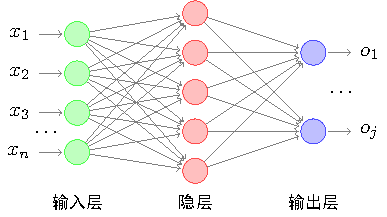
\includegraphics[width=0.6\textwidth]{fig08.pdf}
    \caption{三层BP网拓扑结构}
    \label{tri}
  \end{figure}
\end{frame}

\begin{frame}{传递函数——Sigmoid函数}
  \begin{itemize}
  \item 非线性变换函数,又称S型函数
  \item 特点:函数本身及其导数都是连续的
  \end{itemize}
  \begin{columns}[t]
    \column{.4\textwidth}
    \begin{block}{单极性S型函数}
      \[
      f(\chi)=\frac1{1+e^{-\chi}}
      \]
      \centering
      \begin{figure}
        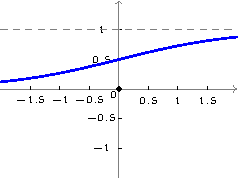
\includegraphics{fig09.pdf}
      \end{figure}
    \end{block}

    \column{.4\textwidth}
    \begin{block}{双极性S型函数}
      \[
      f(\chi)=\frac{1-e^{-\chi}}{1+e^{-\chi}}
      \]
      \centering
      \begin{figure}
        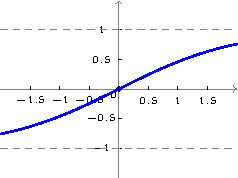
\includegraphics{fig10.pdf}        
      \end{figure}
    \end{block}
  \end{columns}
\end{frame}

\begin{frame}{传统BP学习算法}
  以三层感知器[figure \alert{\ref{tri}}]为例。

  1. 网络误差与权值调整

  当网络输出与期望输出不等时,存在输出误差$E$,定义如下
  \begin{equation}
    \begin{array}{ll}
      E &=\frac{1}{2}(d-O)^2 \\
      &=\frac{1}{2}\sum_{\kappa=1}^\ell(d_k-o_k)^2
    \end{array}
  \end{equation}
  将以上误差定义式展开至隐层,有
  \begin{equation}
    \begin{array}{ll}
      E &=\frac{1}{2}\sum_{\kappa=1}^\ell[d_{\kappa}-f(net_\kappa)]^2 \\
      &=\frac{1}{2}\sum_{\kappa=1}^\ell[d_{\kappa}-f(\sum_{j=0}^m\omega_{j\kappa}y_j)]^2
    \end{array}
  \end{equation}
\end{frame}

\begin{frame}{传统BP学习算法}
  进一步展开至输入层,有
  \begin{equation}
    \begin{array}{ll}
      E &=\frac{1}{2}\sum_{\kappa=1}^\ell{d_{\kappa}-f[\sum_{j=0}^m\omega_{j\kappa}f(net_j)]}^2 \\
      &=\frac{1}{2}\sum_{\kappa=1}^\ell{d_{\kappa}-f[\sum_{j=0}^m\omega_{j\kappa}f(\sum_{j=0}^n\upsilon_{ij}\chi_i)]}^2
    \end{array}
  \end{equation}
  由上式可以看出,网络输入误差是各层权值$\omega_{j\kappa}$、%
  $\upsilon_{ij}$的函数,因此调整权值可改变误差$E$。

  显然,调整权值的原则是\alert{使误差不断减小},因此应使权值与误差的梯度%
  下降成正比,即

  \begin{equation}
    \begin{array}{lll}
      \Delta \omega_{j\kappa}=-\eta \frac{\partial E}{\partial \omega_{j\kappa}} & j=0,1,2,\ldots,m; & \kappa=1,2,\ldots,\ell
    \end{array}
  \end{equation}

  \begin{equation}
    \begin{array}{lll}
      \Delta \upsilon_{ij}=-\eta \frac{\partial E}{\partial \upsilon_{ij}} & i=0,1,2,\ldots,n; & j=1,2,\ldots,m
    \end{array}
  \end{equation}

\end{frame}

\begin{frame}{传统BP学习算法}
  对于一般多层感知器,设共有$h$个隐层,按前向顺序各隐层节点数分别记为%
  $m_1,m_2,\ldots,m_h$,各隐层输出分别记为$y^1,y^2,\ldots,y^h$,%
  各层权值矩阵分别记为$W^1,W^2,\ldots,W^h,W^h+1$,则各层权值调整公式%
  为

  输出层
  \begin{equation}
    \begin{array}{lll}
      \scriptstyle\Delta \omega_{j\kappa}^{h+1}=\eta \delta_{\kappa}^{h+1}y_j^h=\eta(d_\kappa-o_\kappa)o_\kappa(1-o_\kappa)y_j^\kappa & \scriptstyle j=0,1,2,\ldots,m_h; & \scriptstyle \kappa=1,2,\ldots,\ell
    \end{array}
  \end{equation}
  第$h$隐层
  \begin{equation}
    \begin{array}{lll}
      \scriptstyle\Delta \omega_{ij}^{h}=\eta \delta_j^hy_i^h-1=\eta(\sum _{\kappa=1}^l \delta_\kappa^o\omega_{j\kappa}^{h+1}y_j^\kappa(1-y_j^kappa)y_i^h-1 & \scriptstyle i=0,1,2,\ldots,m_(h-1); & \scriptstyle j=1,2,\ldots,m_h
    \end{array}
  \end{equation}
\end{frame}

\begin{frame}{传统BP学习算法}
  按以上规律逐层类推,则第一隐层权值调整公式
  \begin{equation}
    \begin{array}{lll}
      \scriptstyle \Delta \omega_{pq}^1=\eta \delta_q^1\chi_p=\eta(\sum_{r=1}^{m_{2}}\delta_r^2\omega_{qr}^2)y_q^1(1-y_q^1)\chi_p & \scriptstyle p=0,1,2,\ldots,n; & \scriptstyle j=1,2,\ldots,m_1
    \end{array}
  \end{equation}
  容易看出,BP学习算法中,\alert{各层权值调整公式形式上都是一样}%
  的,均由3个因素决定,即:
  \begin{itemize}
  \item 学习率$\eta$
  \item 本层输出的误差信号$\delta$
  \item 本层输入信号$Y$%(或$X$)。
  \end{itemize}
  其中输入层误差信号与网络的期望输出与实际输出之差有关,直接反应了%
  输出误差,而各隐层的误差信号与前面各层的误差信号有关,是\alert{%
    从输出层开始逐层反传过来的}。
\end{frame}


\begin{frame}{传统BP学习算法}
  \begin{itemize}
  \item 可以看出BP算法\alert{属于$\delta$学习规则类},这类算法%
    常被称为\alert{误差的梯度下降算法}。
  \item $\delta$学习规则可以看成是Widrow-Hoff(LMS)学习规则的一%
    般化(generalize)情况。LMS学习规则与神经元采用的变换函数无关,%
    因而不需要对变换函数求导,$\delta$学习规则则没有这个性质,要求变换%
    函数可导。
  \end{itemize}
\end{frame}

\begin{frame}{改进的BP学习算法}
  标准的BP算法在应用中暴露出不少内在的缺陷:
  \begin{itemize}
  \item 极易形成局部最小而得不到全局最优;
  \item 学习效率低,收敛速度慢;
  \item 隐节点的选取缺乏理论指导;
  \item 训练时学习新样本有遗忘旧样本的趋势。
  \end{itemize}
\end{frame}

\begin{frame}{改进的BP学习算法}
  针对上述问题,国内外已提出不少有效的改进算法。
  \begin{itemize}
  \item 引入动量因子(收敛速度);
  \item 引入自适应调节学习率(收敛速度);
  \item 引入陡度因子(收敛速度);
  \item 采用总体样本批训练法(遗忘旧样本);
  \item 模拟退火算法、遗传算法等全局优化算法(局部极小点);
  \item \ldots
  \end{itemize}
\end{frame}

\begin{frame}{总结:BP网络的三要素}
  \centering
  \begin{figure}
    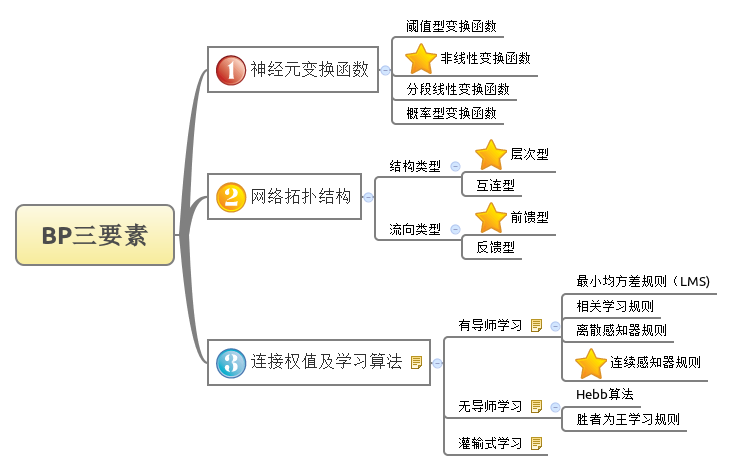
\includegraphics[width=.8\textwidth]{fig11.png}
    \caption{BP网络的三要素}
    \label{fig:bp3elements}
  \end{figure}
\end{frame}


\begin{frame}{BP网的功能}
  BP网是至今为止应用最广泛的神经网络

  \begin{itemize}
  \item
    非线性映射能力
  \item
    泛化能力
  \item
    容错能力
  \end{itemize}
\end{frame}

\section{其他网络综述}
\label{sec:other}

\begin{frame}{其他网络综述}
    \vspace{-1em}
  \begin{figure}
    \centering
    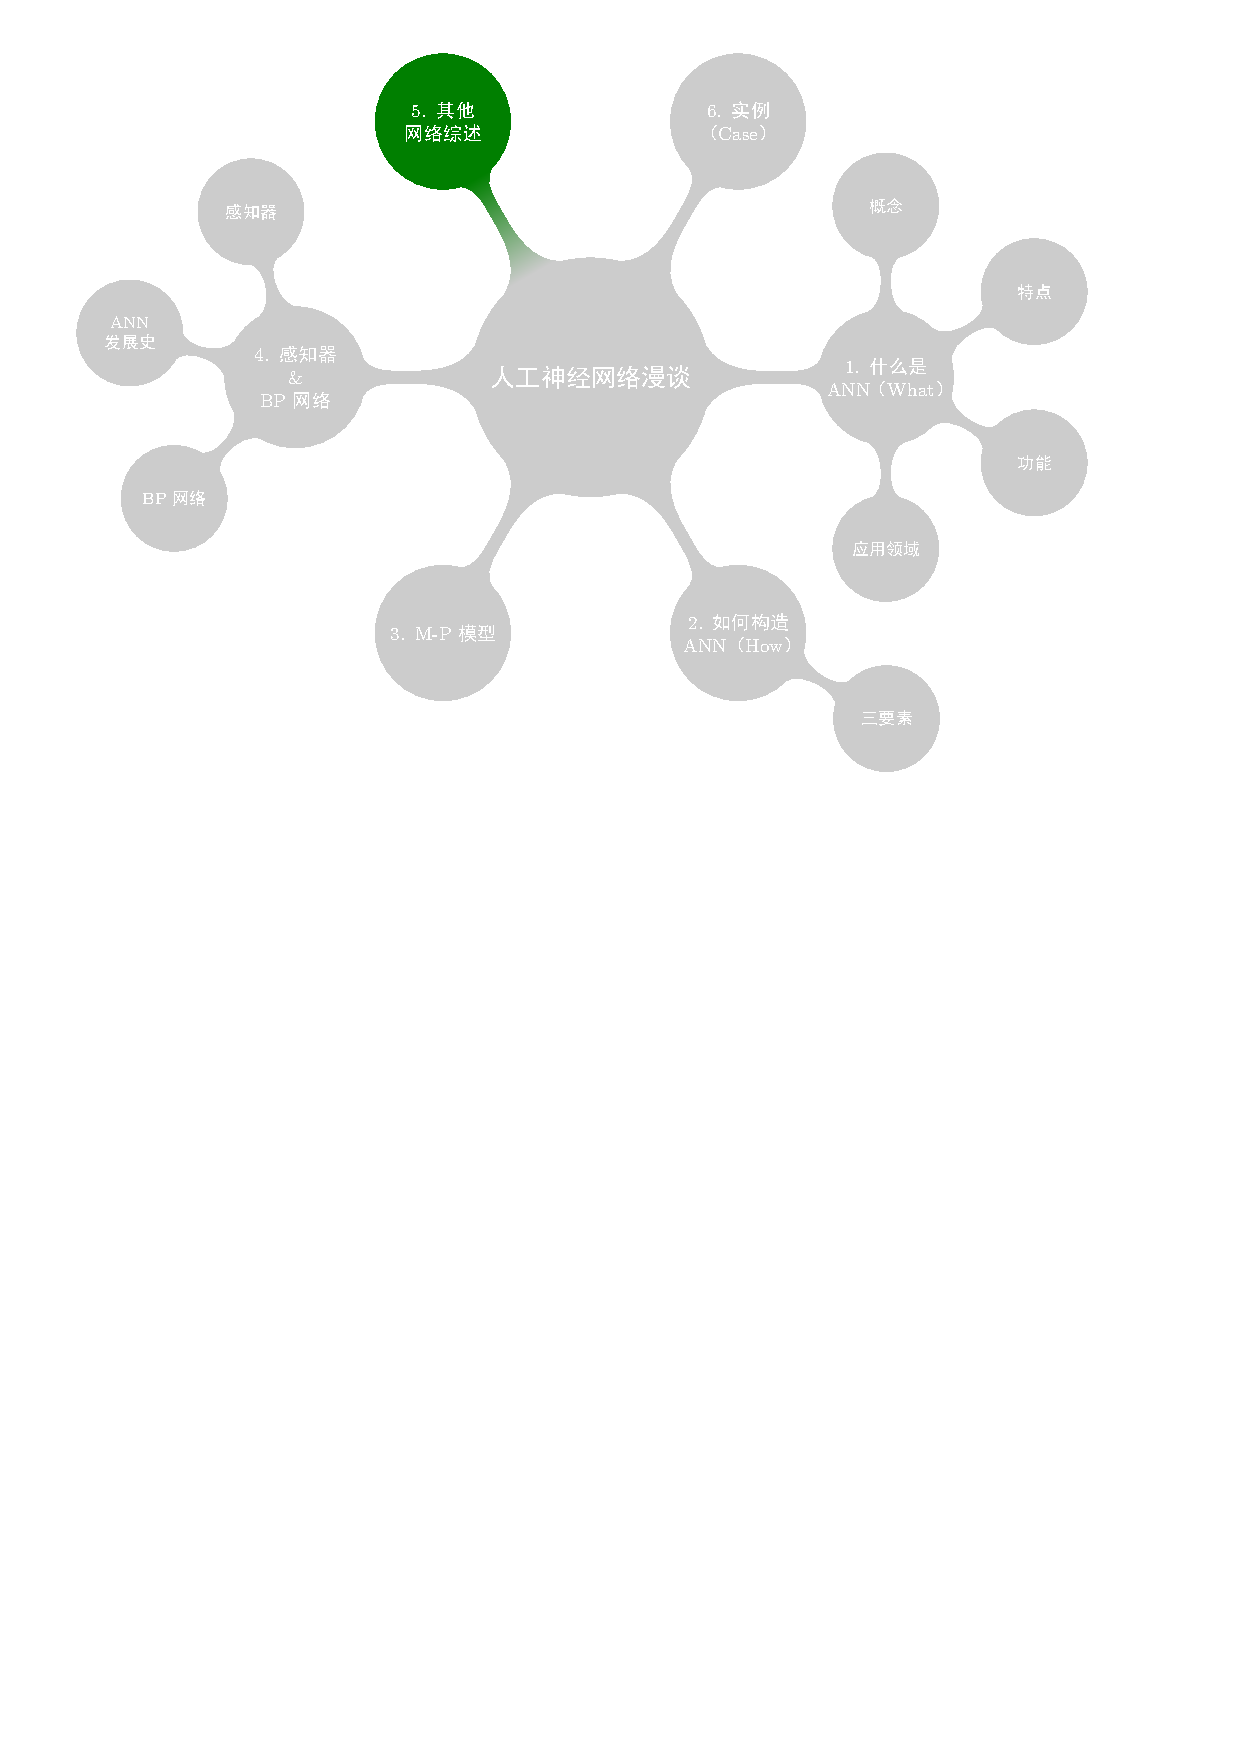
\includegraphics[width=\textwidth]{mindmap/map6.pdf}
  \end{figure}
\end{frame}


\begin{frame}[allowframebreaks]{人工神经网络概览}
  下表列出了神经网络发展过程中起过重要作用的十几种著名神经网络的
  情况,它也是神经网络发展史的一个缩影。

    \centering
    %\caption{对神经网络发展有重要影响的神经网络}
    \scriptsize
    
    \begin{longtable}{p{5em}|p{5em}|c|p{6em}|p{6em}|p{8em}}
      \hline
      名称 & 提出者 & 诞生年 & 典型应用领域 & 弱点 & 特点\\
      \hline
      Perceptron(感知器) & Frank Rosenblatt(康奈尔大学) & 1937 & 文字识别、
      声音识别、声纳信号识别、学习记忆问题研究。 & 不能识别复杂字形,对字的大小、
      平移和倾斜敏感。 & 最早的神经网络,已很少应用,有学习能力,只能进行线性分
      类。\\
      \hline
      Adaline(自适应线性单元)和Madaline(多个Adaline的组合网络) & Bernard Widrow
      (斯坦福大学) & 1960--1962 & 雷达天线控制,自适应回波抵消、适应性调制解调、
      电话线中适应性补偿等。 & 要求输入 - 输出之间为线性关系。 & 学习能力较强,较
      早开始商业应用,Madaline是Adaline的功能扩展。\\
      \hline
      Avalanche(雪崩网) & S. Drossberg(波士顿大学) & 1967 & 连续语音识别,机
      器人手臂运动的教学指令 & 不易改变运动速度和插入运动。\\
      \hline
      Cerellatron(小脑自动机) & D.Marr(麻省理工学院) & 1969-1982 & 控制机器
      人的手臂运动 & 需要复杂的控制输入 & 类似于Avalanche网络,能调和各种指令序
      列,按需要缓慢地插入动作。\\
      \hline
      Back Propagation(误差反传网络) & P. Werbos(哈佛大学)David
      Rumelhart(斯坦福大学)James McClelland(斯坦福大学) & 1974--1985 & 语音
      识别、工业过程控制、贷款信用评估、股票预测、自适应控制等 & 需要大量输入 - 输
      出数据,训练时间长,易陷入局部极小。 & 多层前馈网络,采用最小均方差学习方
      式,是应用最广泛的网络。\\
      \hline
      Adaptive Resonance Theory(自适应共振理论ART)有ART \Rmnum{1}、ART
      \Rmnum{2}和ART \Rmnum{3}3种类型 & G.Carpenter和S.Grossberg(波士顿大学) &
      1976--1990 & 模式识别领域,擅长识别复杂模式或未知的模式 & 受平移、旋转及尺
      度的影响。系统比较复杂、难以用硬件实现。 & 可以对任意多和任意复杂的二维模
      式进行自组织学习, ART \Rmnum{1}用于二进制,ART \Rmnum{2}用于连续信号。 \\
      \hline
      Brain State in a Box(盒中脑BSB网络) & James Anderson(布朗大学) & 1977
      & 解释概念形成,分类呵知识处理 & 只能作一次性决策,无重复性共振。 & 具有最
      小均方差的单层自联想网络,类似于双向联想记忆,可对片段输入补全。 \\
      \hline
      Neocognition(新认知机) & Fukushima K 福岛邦彦(日本广播协会) &
      1978--1984 & 手写字母识别 & 需要大量加工单元和联系 & 多层结构化字符识别网
      络,与输入模式的大小、平移和旋转无关,能识别复杂字形。\\
      \hline
      Self-Organizing feature map(自组织特征映射网络) & Toevo Konhonen(芬兰赫
      尔辛基技术大学)&1980&语音识别,机器人控制,工业过程控制,图像压缩,专家系
      统等。& 模式类型数据预先知道。 & 对输入样本自组织聚类,映射样本空间的分布。
      \\
      \hline
      Hopfield网络 & John Hopfield (加州理工学院) & 1982 & 求解TSP问题,线性规
      划,联想记忆和用于辨识。 & 无学习能力,连接要对称,权值要预先给定。 & 单层
      自联想网络,可从有缺损或有噪声输入中恢复完整信息。\\
      \hline
      Boltzman machine(玻耳兹曼机) Cauchy machine(柯西机) & J.Hinton(多伦多
      大学)T.Sejnowaski(霍布金斯大学) & 1985--1986 & 图像、声纳和雷达等模式
      识别。& 玻耳兹曼机训练时间长,柯西机在某些统计分布下产生噪声。 & 一种采用
      随机学习算法的网络,可训练实现全局最优。\\
      \hline
      Bidirectional Associative Memory(BAM,双向联想记忆网) & Bart Kosko(南加
      州大学) & 1985--1988 & 内容寻址的联想记忆 & 存储的密度低,数据必须适应编
      码。 & 双向联想式单层网络,具有学习功能,简单易学。 \\
      \hline
      Counter Proagation(CPN,双向传播网) & Robert Hecht-Nielsen & 1986 & 神经
      网络计算机,图像分析和统计分析。 &  需要大量处理单元和连接,需要高度准确。
      & 一种在功能上作为统计最优化和概率密度函数分析的网络。\\
      \hline
      Radial Basis Functions(RBF,径向基函数网络) & Broomhead Lowe & 1988 & 非
      线性函数逼近,时间序列分析,模式识别、信息处理、图像处理、系统建模。 & 需
      要大量输入输出数据,计算较复杂。 & 网络设计采用原理化方法,有坚实的数学基
      础。\\
      \hline
      Support Vector Machine(SVM,支持向量机) & Vapmk & 1992--1998 & 模式分类,非线性映射 &
      训练时间长,支持向量的选择较困难,学习算法的推导较深奥。 & 在模式分类问题
      上能提供良好的泛化性能。\\
      \hline
    \end{longtable}
    
  \end{frame}

\section{实例}
\label{sec:case}

\begin{frame}{实例}
    \vspace{-1em}
  \begin{figure}
    \centering
    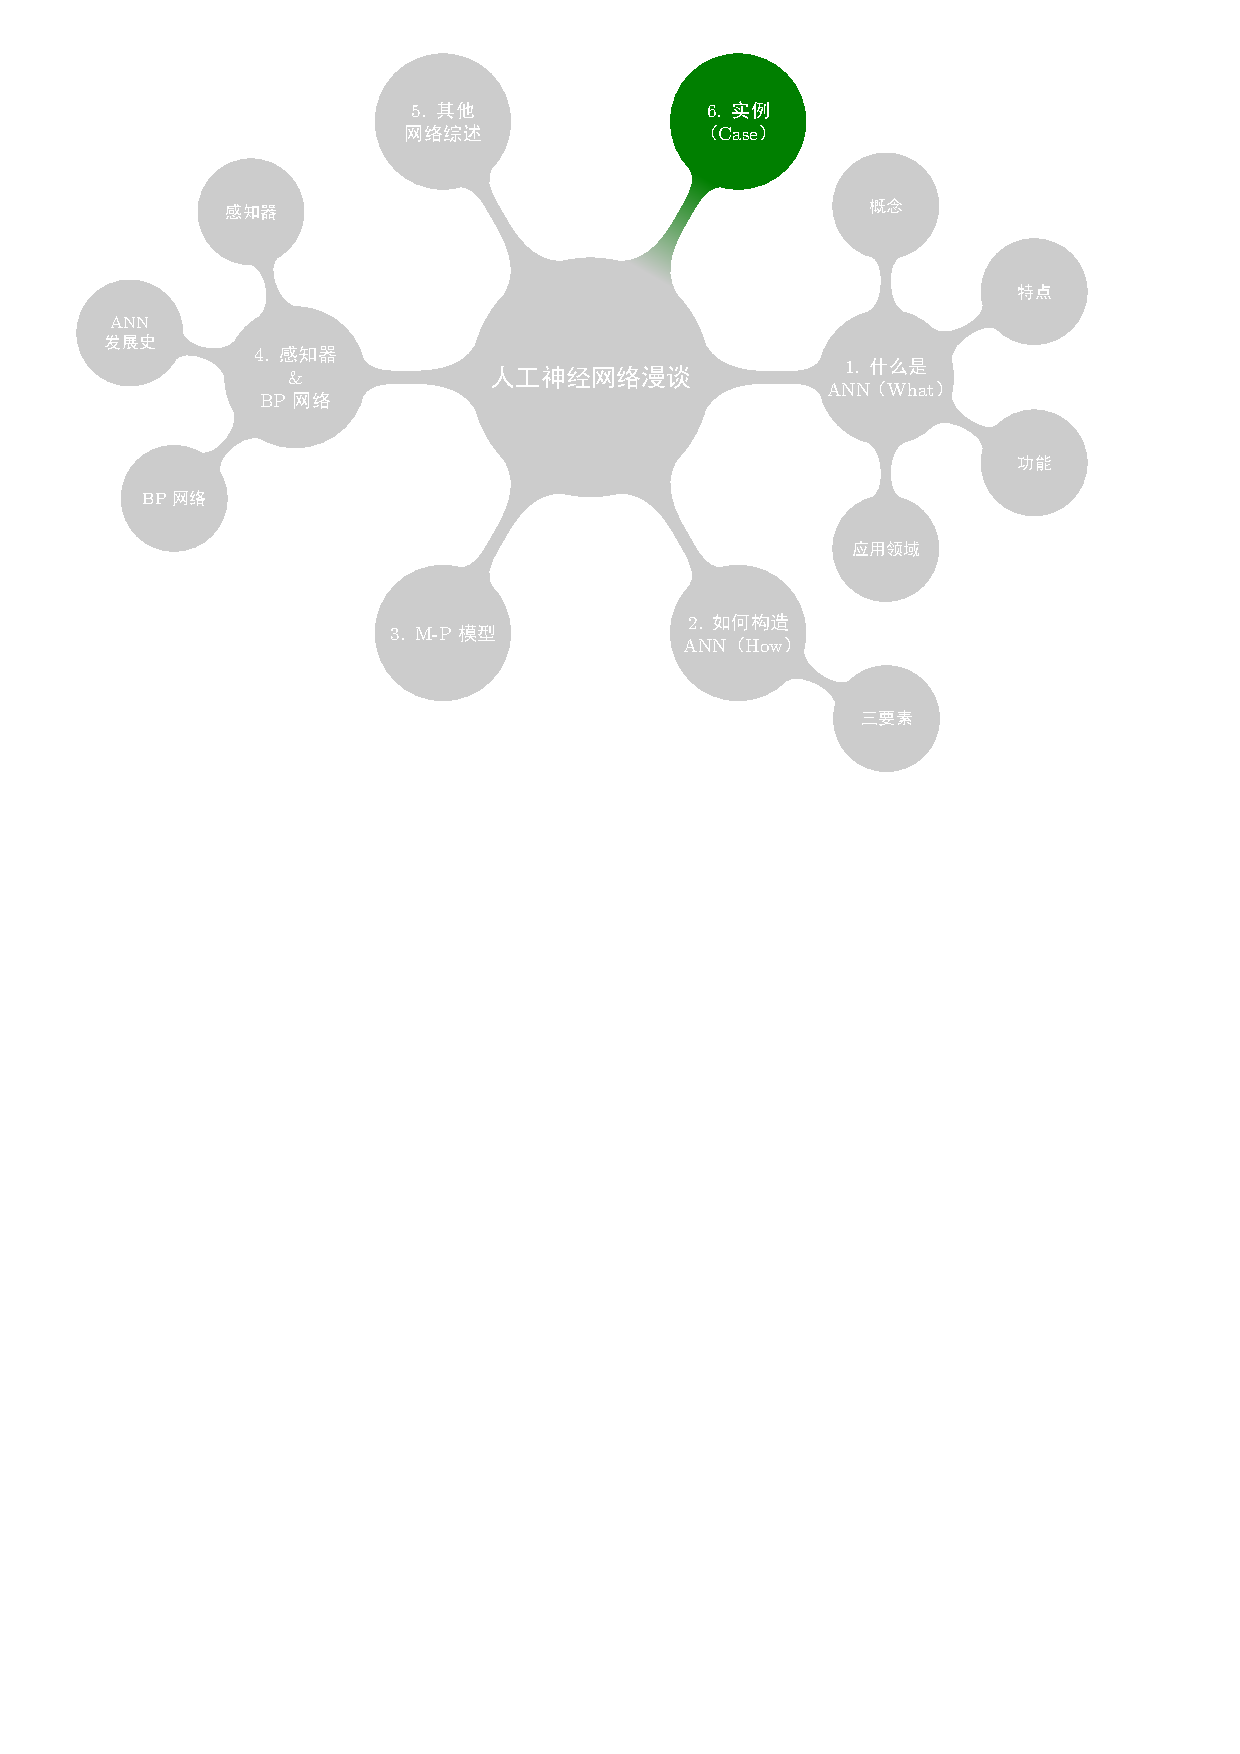
\includegraphics[width=\textwidth]{mindmap/map7.pdf}
  \end{figure}
\end{frame}

\begin{frame}{怎么应用ANN解决问题?}
  在使用ANN解决实际问题前,你应该先问自己下面几个问题:
  \begin{enumerate}
  \item 什么时候可以用神经网络?
  \item 分类还是回归?
  \item 确定的还是随机的?
  \item 有监督还是无监督?
  \item 在线还是离线?
  \item PC还是其他硬件设备(DSP芯片)?
  \end{enumerate}
\end{frame}
  
\begin{frame}{CASE \Rmnum{1} 曲线拟合}
  \begin{itemize}
  \item 背景介绍:BP网络采用非线性传递函数,相对线性网络具有%
    更强的拟合能力,因此对于现实中遇到的各种复杂的函数波形可以进%
    行很好的逼近。
  \item 实例要求:对一个具有一定采样率的正弦函数用BP网络来逼近%
    其波形。
  \end{itemize}
  \begin{exampleblock}{正弦信号}
    \centering
    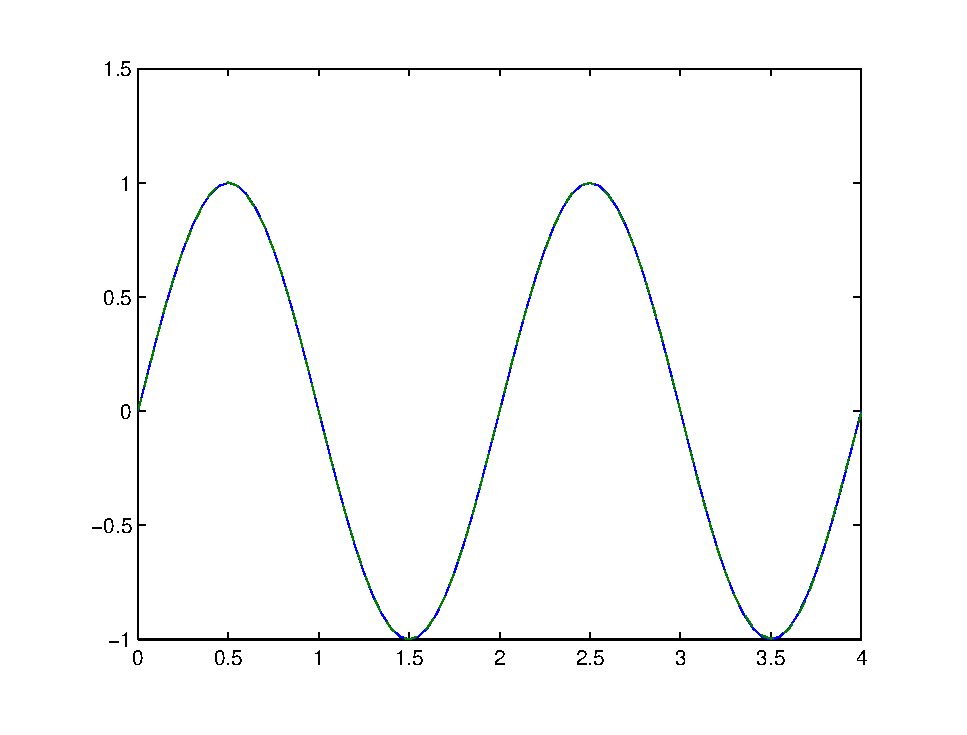
\includegraphics[width=4cm]{fig12.eps}
  \end{exampleblock}
\end{frame}

\begin{frame}{CASE \Rmnum{2} 特征识别}
  \begin{itemize}
  \item 背景介绍:利用计算机进行模式识别是一项很有用的技术,尤其%
    是利用机器来识别图形符号的特征。
  \item 实例要求:设计并训练一个BP网络,完成26个字母的图像识别。
    \begin{exampleblock}{三层BP网拓扑结构}
      \centering
      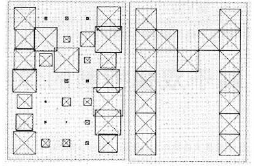
\includegraphics[width=4cm]{fig13.png}
    \end{exampleblock}
  \end{itemize}
\end{frame}


\begin{frame}
  \begin{center}
    \Huge{\textcolor{red}{Thank You!}}
  \end{center}
\end{frame}

\end{document}}

